%% 
%% Copyright 2019-2024 Elsevier Ltd
%% 
%% This file is part of the 'CAS Bundle'.
%% --------------------------------------
%% 
%% It may be distributed under the conditions of the LaTeX Project Public
%% License, either version 1.3c of this license or (at your option) any
%% later version.  The latest version of this license is in
%%    http://www.latex-project.org/lppl.txt
%% and version 1.3c or later is part of all distributions of LaTeX
%% version 1999/12/01 or later.
%% 
%% The list of all files belonging to the 'CAS Bundle' is
%% given in the file `manifest.txt'.
%% 
%% Template article for cas-dc documentclass for 
%% double column output.

\documentclass[a4paper,fleqn]{cas-dc}

% If the frontmatter runs over more than one page
% use the longmktitle option.

%\documentclass[a4paper,fleqn,longmktitle]{cas-dc}
\usepackage{amsmath,amsfonts}
\usepackage{amsthm}
\usepackage{algorithmic}
\usepackage{algorithm}
\usepackage{array}
\usepackage{textcomp}
\usepackage{stfloats,siunitx}
\usepackage{url}
\usepackage{verbatim}
\usepackage{graphicx}
%\usepackage{newtxtext}
\usepackage{graphicx}
\graphicspath{{figs/}}
\usepackage{cite,soul}
\usepackage{multirow,booktabs}
\usepackage{float,booktabs,threeparttable} 
\usepackage{tikz,graphics,color,fullpage,float,epsf,caption,subcaption}
\usepackage{epsfig,epstopdf,arydshln,amssymb,multirow,microtype,amsthm,amsfonts}



\usepackage[numbers]{natbib}
%\usepackage[authoryear]{natbib}
%\usepackage[authoryear,longnamesfirst]{natbib}

%%%Author macros
\def\tsc#1{\csdef{#1}{\textsc{\lowercase{#1}}\xspace}}
\tsc{WGM}
\tsc{QE}
%%%

% Uncomment and use as if needed
%\newtheorem{theorem}{Theorem}
%\newtheorem{lemma}[theorem]{Lemma}
%\newdefinition{rmk}{Remark}
%\newproof{pf}{Proof}
%\newproof{pot}{Proof of Theorem \ref{thm}}

\begin{document}
\let\WriteBookmarks\relax
\def\floatpagepagefraction{1}
\def\textpagefraction{.001}

% Short title
\shorttitle{}    

% Short author
%\shortauthors{P. Junsawang et~al.}  

% Main title of the paper
\title [mode = title]{Online Bootstrapping for Streaming Data Environment with Limited Storage
by Upper-Lower-End Interval Re-sampling}  

% Title footnote mark
% eg: \tnotemark[1]
\tnotemark[1] 

% Title footnote 1.
% eg: \tnotetext[1]{Title footnote text}
\tnotetext[1]{} 

% First author
%
% Options: Use if required
% eg: \author[1,3]{Author Name}[type=editor,
%       style=chinese,
%       auid=000,
%       bioid=1,
%       prefix=Sir,
%       orcid=0000-0000-0000-0000,
%       facebook=<facebook id>,
%       twitter=<twitter id>,
%       linkedin=<linkedin id>,
%       gplus=<gplus id>]

%\author[1]{P. Junsawamg}%[<options>]
%
%% Corresponding author indication
%%\cormark[1]
%
%% Footnote of the first author
%%\fnmark[1]
%
%% Email id of the first author
%\ead{jpremlc@gmail.com}
%
%% URL of the first author
%%\ead[url]{}
%
%% Credit authorship
%% eg: \credit{Conceptualization of this study, Methodology, Software}
%%\credit{}
%
%% Address/affiliation
%\affiliation[1]{organization={Advanced Virtual and Intelligent Computing (AVIC) Research Center, Department of Mathematics and Computer Science, Chulalongkorn University},
%            addressline={}, 
%            city={Bangkok},
%%          citysep={}, % Uncomment if no comma needed between city and postcode
%            postcode={10330}, 
%            state={},
%            country={Thailand}}
%
%
%
%% URL of the second author
%%\ead[url]{}
%
%% Credit authorship
%%\credit{}
%
%% Address/affiliation
%%\affiliation[2]{organization={},
%%            addressline={}, 
%%            city={},
%%          citysep={}, % Uncomment if no comma needed between city and postcode
%%            postcode={}, 
%%            state={},
%%            country={}}
%\author[1]{S. Phimoltares}
%\cormark[1]
%
%% Corresponding author text
%\cortext[1]{Corresponding author}
%\ead{suphakant.p@chula.ac.th}
%
%\author[1]{C. Lursinsap}%[]
%
%% Footnote of the second author
%%\fnmark[2]
%
%% Email id of the second author
%\ead{chidchanok.L@chula.ac.th}


% Footnote text
%\fntext[1]{}

% For a title note without a number/mark
%\nonumnote{}

% Here goes the abstract
\begin{abstract}
Bootstrapping has been widely used as an effective %proven the most appropriate 
non-parametric approach to estimate the population 
variance by resampling the entire sample with replacement. This approach does not make any 
assumption about the probability distribution of data, making it suitable for several real applications. 
Although it is very efficient and practical, the method cannot be applied to streaming data with limited memory due to the risk of data overflow.
Furthermore, it is impossible to apply conventional
bootstrapping to estimate the variance of data features in machine learning using the  
{\em discard-after-learn concept}, in which the learned data are entirely discarded afterwards. Recently, there have been
few methods attempting to apply conventional bootstrapping to streaming data, which require pre-defined 
parameters and the assumption of normal distribution, which may not conform with the actual distribution 
of data. This paper proposes a new method called Recursively Bootstrapping at Upper-Lower Tails (RBULT) 
to cope with chunk-wise data in a streaming environment. Only the current incoming data is bootstrapped 
without any assumption on data probability distribution, information from previous chunks, and pre-defined 
parameters. Experimental results on ten simulated continuous streaming datasets with various probability 
distributions and four real-world datasets of multiple chunk sizes (50, 100, and 500) without and with 
outlier contamination levels (0.05\% of population size) show that RBULT significantly outperform
the conventional bootstrapping. In addition, the population variance
estimated by RBULT is closer to the true population variance than the conventional bootstrapping method. 
%Here goes the abstract \nocite{*}%% Remove this line from your manuscript.
\end{abstract}

% Use if graphical abstract is present
%\begin{graphicalabstract}
%\includegraphics{}
%\end{graphicalabstract}

% Research highlights
\begin{highlights}
\item We proposed a novel methodology called Recursively Bootstrapping at Upper-Lower Tails (RBULT), designed to address the significant limitations of conventional bootstrapping in streaming data environments.
\item A two-phase recursive process that compares incoming data histograms against standard distribution shapes to automatically extend boundary intervals.
\item The integration of a z-score-based outlier elimination algorithm, which ensures valid range estimates even in contaminated streaming environments where traditional methods often fail.
\item Comprehensive testing across ten simulated distributions and four real-world datasets, demonstrating that RBULT significantly outperforms traditional bootstrapping in range approximation accuracy.
\end{highlights}


%\nocite{*}

% Keywords
% Each keyword is seperated by \sep
\begin{keywords}
 Online Bootstrapping \sep Recursive Re-sampling \sep Limited Memory Environments\sep Streaming Data Environment\sep
\end{keywords}

\maketitle

% Main text
\section{Introduction}\label{sec1_intro}
Bootstrap method is a powerful and widely used statistical tool for estimating uncertainty 
from finite samples across a wide range of parameters, %for any parameter of interest, 
including standard errors, confidence intervals, and 
accuracy measures. Efron \cite{efron} introduced the bootstrap method as a generalisation of the Jackknife 
method, demonstrating that the Jackknife could be mathematically expressed as a linear approximation 
of the bootstrap. The empirical results showed that the proposed methods could effectively estimate the 
standard errors of complex estimators, establishing the foundation for modern resampling techniques.  
Building upon this foundation work, Efron and Tibshirani \cite{efron2} further explored the basic 
concepts and applications of bootstrap methods for estimating standard errors, confidence intervals, 
and other measures of statistical accuracy. 
In standard error estimation, data from a population are resampled with replacement to 
create multiple bootstrap samples, enabling the calculation of statistics and their corresponding standard deviations. 
%for each sample. 
Their results demonstrated that bootstrap estimations provided reasonably accurate and 
efficient alignment with theoretical density curves. Regarding confidence intervals, they empirically 
tested several methods. They found that bootstrap confidence intervals are more precise than standard 
methods, particularly when the statistical distribution deviates from normality. However, achieving 
accurate results typically requires a sufficiently large number of bootstrap replications. Subsequent studies have further 
refined the practical implementation of bootstrap methods in applied research. Carpenter and Bithell 
\cite{carpenter} presented a comprehensive guide for applying 
bootstrap confidence intervals in health care data, systematically addressing when, which, and how to 
implement these methods. They evaluated various bootstrap approaches for confidence intervals across 
three distinct families: pivotal, non-pivotal, and test-inversion methods. Their experimental analysis 
concluded that bootstrap confidence intervals serve as a suitable alternative when the assumptions 
underlying traditional distributional methods do not hold, such as asymptotic normality, particularly in 
scenarios involving small sample sizes or complex data structures.

Range estimation in univariate data sets constitutes a fundamental component of statistical analysis and 
computational modeling, particularly in determining the spread between minimum and maximum observations. 
\cite{wood} introduced a novel re-sampling methodology for establishing control limits in statistical 
process control charts, demonstrating significant advances over traditional parametric approaches across 
multiple chart types, including those monitoring means, ranges, standard deviations, medians, 
proportion defective, and defect counts. The methodology operates through a systematic process of 
aggregating observed data, generating multiple bootstrap samples with replacement, computing the 
target statistic for each sample, and deriving the control limits from the empirical percentiles of 
resulting distribution. This approach offers notable methodological advantages, primarily its conceptual 
accessibility and procedural transparency, as it relies exclusively on random sampling principles and 
percentile calculations, thereby eliminating complex distributional assumptions while maintaining 
statistical rigor and reducing technical prerequisites for implementation. The re-sampling framework 
represents a significant contribution to non-parametric statistical process control, offering robust 
alternatives to conventional approaches that may be sensitive to distributional assumptions or limited 
sample sizes, ultimately enhancing the ability of interpretation for practitioners across diverse 
analytic contexts. Palm and Nagler \cite{palm} presented an online bootstrap method for uncertainty 
quantification in large streams of dependent data, such as time series, directly addressing the 
computational and memory limitations of traditional bootstrap methods in big data and streaming 
environments. No restrictive assumptions about data dependence are made in their method. But some
parameters must be predefined and the type of data distribution must be assumed. 
An auto-regressive sequence of increasingly dependent re-sampling weights was applied, 
allowing for $O(1)$ online updates in both memory and time for the bootstrap average and providing a 
significant computational advantage over the blockwise bootstrap. The authors provided rigorous 
theoretical validation under general conditions, including specific restrictions on time series dependence, 
and empirical demonstration on the effectiveness of their approach in 
reliable uncertainty quantification, even in the presence of complex data dependencies. 
Hall and Yao \cite{hall} addressed the challenge of accurately calibrating coverage for non-parametric 
prediction intervals, highlighting the poor performance of conventional methods, such as the standard 
bootstrap and Jackknife. Both the standard bootstrap and Jackknife methods often fail due to tied values in 
re-samples. Jackknife method, despite being unbiased for true coverage, unexpectedly increases 
coverage error, rendering it ineffective for this specific calibration problem. To overcome these 
limitations, the authors propose two primary approaches: interpolation among adjacent order statistics 
and, more significantly, the use of a smoothed version of the bootstrap. These techniques were designed 
to reduce coverage error substantially. The smoothed bootstrap, with an empirically selected bandwidth, 
effectively improves the coverage accuracy and mitigates fluctuations, particularly demonstrating its 
strength in scenarios with small sample sizes. Basically, for conducting the bootstrap method, all 
data were used to repeatedly random selection to approximate a range or other statistical parameters. 
However, in many real-world applications, a single time for conducting the bootstrap, 
data are collected incrementally. This paper proposes a new method called Recursively Bootstrapping at 
Upper-Lower Tails (RBULT) to improve the capabilities of previous methods so as to cope with chunk-wise 
data in a streaming environment. Only the current incoming data is bootstrapped without any assumption on 
data probability distribution, information from previous chunk, and predefined parameters.

The rest of this paper is organised as follows. Section II details the studied problem 
and the objectives of this research. Section III presents the proposed concept of Recursively Bootstrapping 
at Upper-Lower Tails (RBULT) for a streaming environment. Section IV describes the experiments conducted 
to evaluate the performance of our method and discusses the results. Finally, Section V concludes the 
paper with a summary of our findings and suggestions for future work.

\section{Problem Formulation and Constraints}
This section discusses the studied problems under a concerned scenario and constraints which arises in
various online machine learning settings.
  
\subsection{Concerned Scenario}
\label{scenario}
Sampled data continuously flow in forms of chunks into a process, which may be a learning process or
a statistical analyzing process. The size of each chunk is
not fixed and does not exceed %not larger than 
the size of the working memory. Each sampled chunk contains a set of positive
integers whose minimum and maximum values are unknown. The probability distribution of each integer value
is not predefined and unknown. This scenario exists in various problems in machine learning. One of them is 
the problem of training a neural network in a streaming data environment with limited memory size by using 
hyper-ellipsoids \cite{jun}. Estimating the population variance of each feature of incoming data in advance 
can help preemptively expand the size of hyper-ellipsoids to cope with any test set,
leading to improve the accuracy of classification.

\subsection{Studied Problems}
Suppose the size of working memory is fixed at $m$. Let $c_{i}$ be the $i^{th}$ incoming numeric data chunk 
such that $|c_{i}| < m$ and $i \geq 1$. After receiving chunk $c_{i}$ at time $t = i$, the minimum 
and maximum values of population at the left and right ends are estimated. Let $L$ denote the estimated 
left-end value which may be the minimum data value of chunk $c_{i}$ or the minimum value computed from 
bootstrapping some data in $c_{i}$, depending on which one is smaller. Similar to $L$, let $R$ denote the 
estimated right-end value which may be the maximum data value of chunk $c_{i}$ or the maximum value 
computed from bootstrapping some data in $c_{i}$, depending on which one is larger. After estimating $L$ 
and $R$ of $c_{i}$, all data except some partial data at both ends are discarded. Those kept data
are combined with the new incoming data in $c_{i+1}$ for computing new $L$ and $R$.

Figure \ref{example-bootstrap} illustrates an example of the studied problem.  here are three incoming
chunks $c_{1}$, $c_{2}$, and $c_{3}$. $D$ denotes the working memory for accommodating $c_{i}$. Assume that 
the minimum incoming value is 1. At time $t = 1$, the values of $L$ and $R$ are estimated by bootstrapping 
some data of $c_{1}$, setting $L = 3$ and $R = 19$. At time $t = 2$, the values of all data in $c_{2}$ do 
not exceed $L$ and $R$ so no bootstrapping is activated. At time $t = 3$, the values of data in $c_{3}$ 
exceed $L$ and $R$ so $L$ and $R$ are updated. Notice that $L = 1$ is the minimum value so 
no bootstrapping is applied to the left end. Only the value of $R$ is re-estimated by bootstrapping, 
setting $R = 21$.

From the example in Figure \ref{example-bootstrap}, the objective of this study is to estimate the values 
of $L$ and $R$ so that most data in subsequent incoming chunks fall %can lie
within the interval of $\left[ L,R \right]$ with
the minimum number of estimating the values of $L$ and $R$. Therefore, the studied problems defined as 
follows.

\begin{figure}[!h]
\centering
%\resizebox{2.8in}{3.7in}{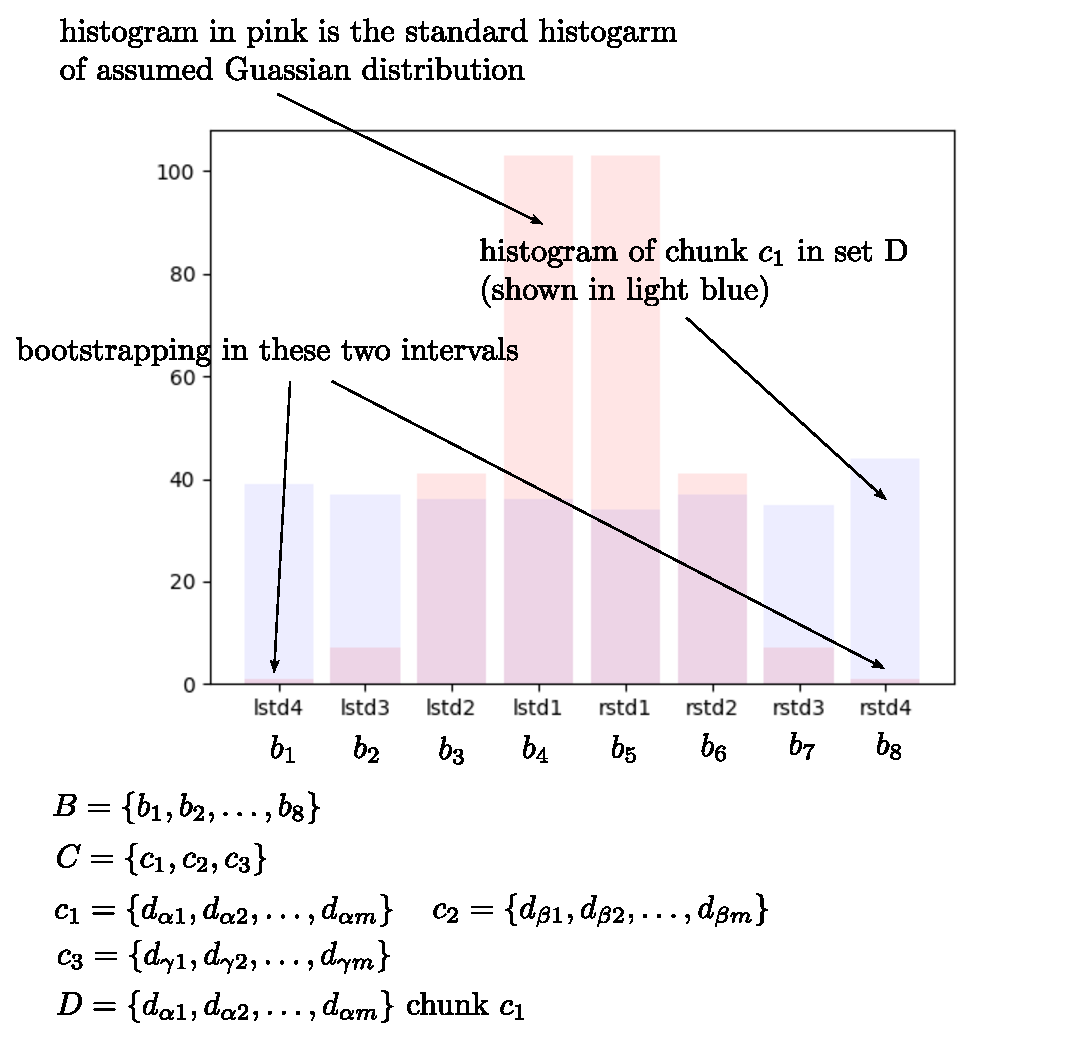
\includegraphics{example-histogram.eps}} 
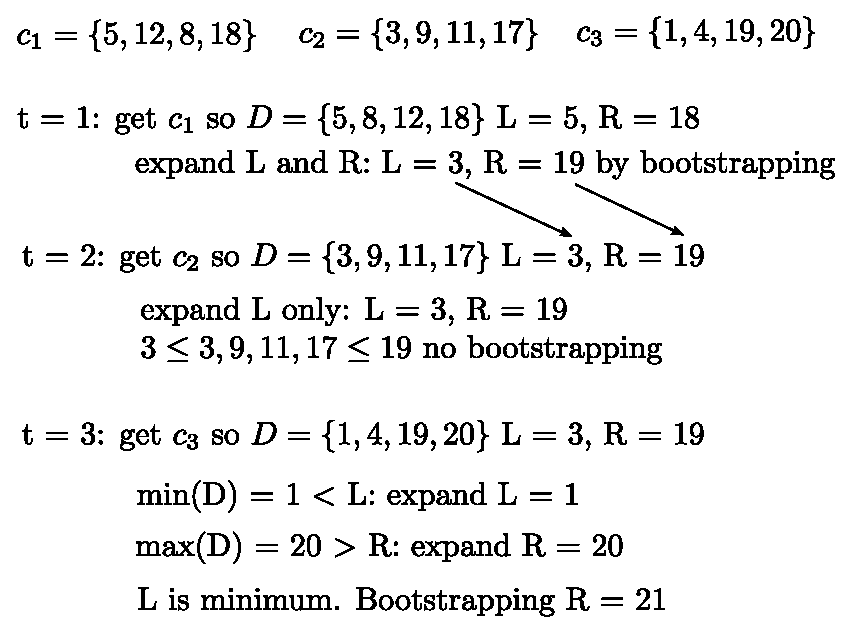
\includegraphics[scale = 0.5]{example-bootstrap.eps} 
\caption{An example of studied problem.} 
\label{example-bootstrap} 
\end{figure}

\begin{enumerate}
\item How to estimate the population variance interval without using the entire data in set $D$ so that the 
data in next incoming chunk always fall within the new interval of estimated 
population variance? After estimation, the almost entire data set should be discarded, making it ready to 
store the next incoming data chunk. 
\item Theoretically, how many times on average must the data interval in set $D$ be expanded according to the 
estimated population variance?
\end{enumerate}

\subsection{Constraints}

Let %$|{\bf c}_i|$ 
$|c_i|$ represent the number of elements in a given chunk, %${\bf c}_i$
$c_i$. The bin %${\bf B}$ 
$B$ is an interval with a left end, $L$, and a right end, $R$. The following constraints apply:

\begin{enumerate}
    \item The probability distribution of each integer, $d_{j}$, within a chunk, %${\bf c}_i$
    $c_i$, is unknown.
    \item The size of a chunk, %$|{\bf c}_{i}|$
    $|c_{i}|$, may or may not be equal to the size of the next chunk, 
    %$|{\bf c}_{i+1}|$
    $|c_{i+1}|$. Furthermore, $|c_{i}| < |D|$.
    \item Once all integers in a chunk, %${\bf c}_{i}$
    $c_{i}$, have been assigned to a bin, the chunk is completely 
    discarded and cannot be reassigned.
\end{enumerate}  

\section{Proposed Concept of RBULT}
\label{concept}
This study does not make any assumption about the probability distribution of incoming data chunk same as
the classical bootstrap method. However, RBULT re-samples the data only in the left-end and right-end 
intervals. This differs from the classical bootstrap method, which re-samples data without location 
constraint. Due to these new re-sampling regions, two consequent problems arise. The first problem
is how large the left-end and right-end intervals should be.

\begin{figure}[!t]
\centering
%\resizebox{2.8in}{3.7in}{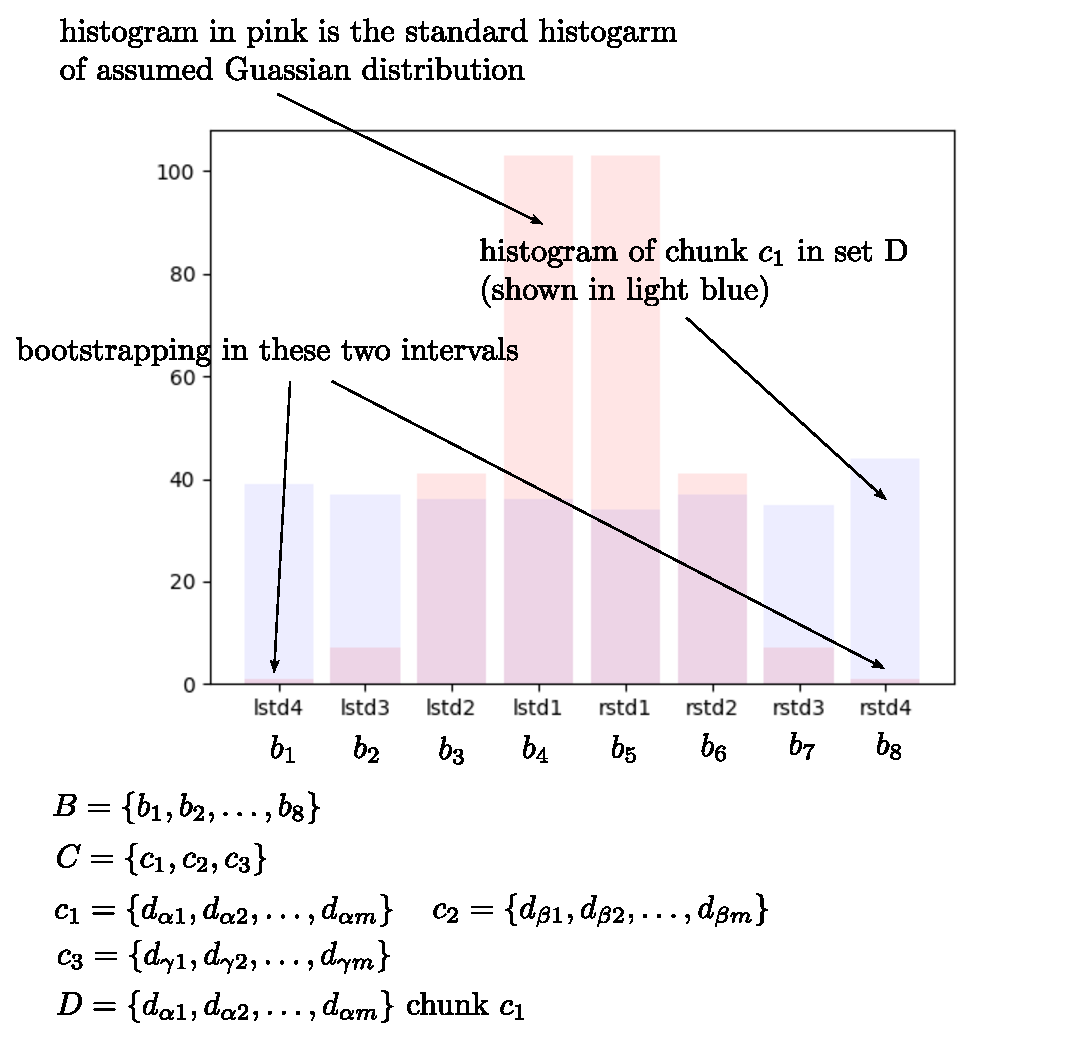
\includegraphics{example-histogram.eps}} 
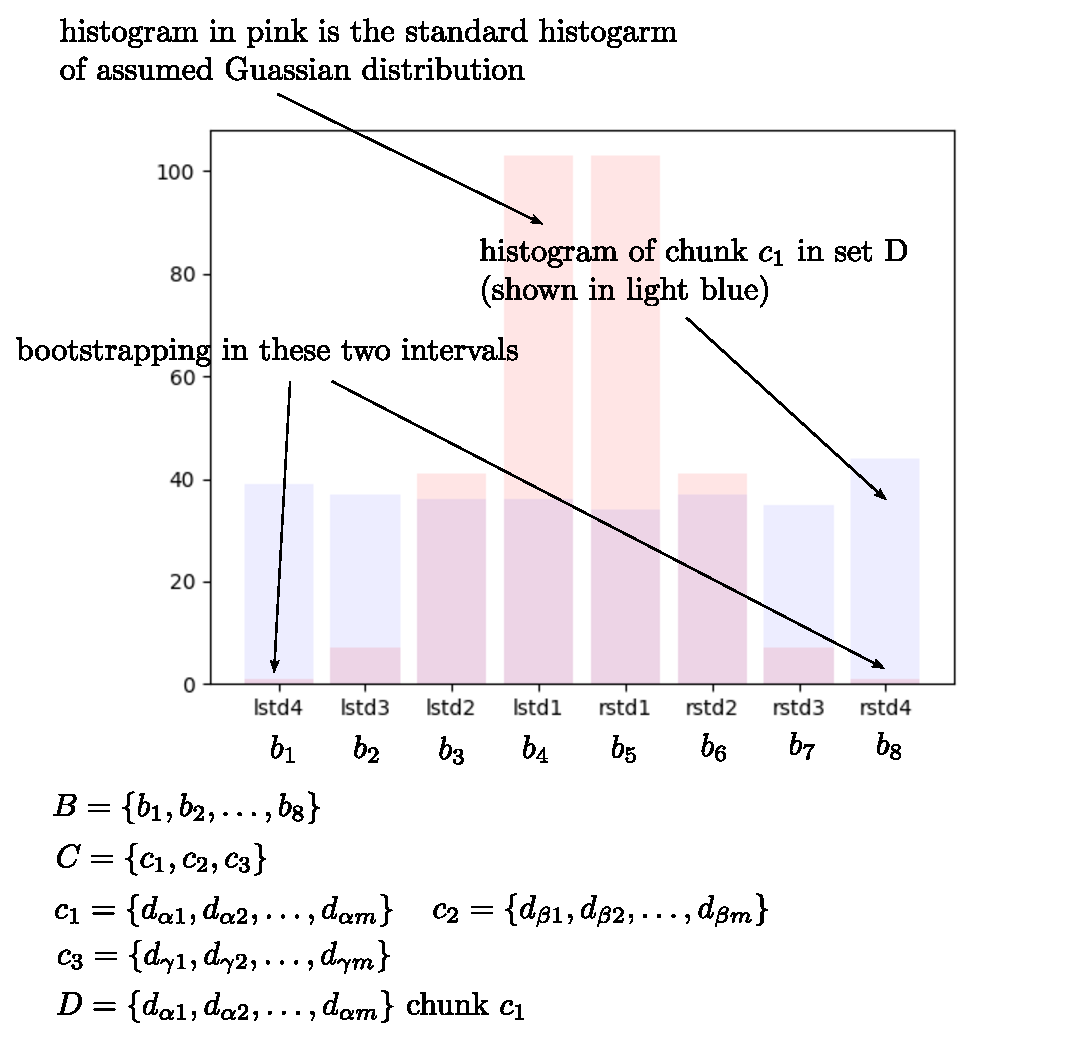
\includegraphics[scale = 0.5]{example-histogram.eps} 
\caption{An example of standard histogram of probabilistic distribution (shown in pink) versus the
data histogram of incoming data distribution (shown in blue color).} 
\label{example-histogram} 
\end{figure}

The size of left-end and right-end intervals are determined from the standard histogram shape of 
probabilistic distribution. If the heights of left-end and right-end intervals in the histogram of 
incoming data distribution %are higher than 
exceed the corresponding heights of the same intervals in
the standard histogram, the left-end and right-end intervals must be extended by bootstrapping the
data in both intervals. Figure \ref{example-histogram} illustrates an example of the standard histogram 
shown in pink color and the data histogram shown in blue color. Clearly, the height of data at the 
left-end and right-end intervals are exceed %higher than the 
those of the standard histogram. There are eight intervals
denoted by $b_{1}$ to $b_{8}$.

The second consequent problem %is which 
concern identifying an appropriate probabilistic distribution %is appropriate 
to solve the first 
problem. The appropriate probabilistic distribution is determined from the first incoming chunk, %This is based on 
under the assumption that %the very 
subsequent incoming chunks possess the same probabilistic 
distribution with small divergence. The experimental results in Section \ref{experiment} confirm that this 
assumption is practically reasonable.


Suppose there are eight intervals in set $B$. The proposed concept has two phases. The first phase analyses 
the probability distribution of the
first incoming data chunk and compare the standard histogram of the distribution with the actual histogram
of the incoming data. If they are different, the data in $b_{1}$ and $b_{8}$ are bootstrapped to 
extend both boundary intervals $b_{1}$ and $b_{8}$. All data not in $b_{1}$ and $b_{8}$ are discarded afterwards. 
The second phase performs the following steps: 
\begin{enumerate}
\item Get a new data chunk and distribute the data into the corresponding intervals. 
\item Compute a new center and partition new set of intervals. 
\item Analyze the probability distribution of data using the new center and new set of intervals. 
\item Compare the height of the standard histogram with that of the actual histogram of the incoming data. If they are 
different, the data in $b_{1}$ and $b_{8}$ are bootstrapped to extend both intervals.
\item Repeat steps 1-4.
\end{enumerate}

Figure \ref{frame-work} illustrates the proposed concept of recurring online bootstrapping.  
A standard histogram, comprising eight bins (highlighted in pink), 
is generated based on a known statistical distribution, where the height of each bin represents the 
theoretical count of elements. The top section of Figure \ref{frame-work} demonstrates that when an expansion is required, the 
number of incoming data points in the leftmost or rightmost intervals (shaded in blue) exceeds the 
theoretical capacity of the standard histogram.
%if the 
%number of incoming data points in the leftmost or rightmost intervals (shaded in blue) exceeds the 
%theoretical capacity of the standard histogram, an expansion is required. 
To address this, the proposed 
recurring online bootstrap method incrementally extends 
the histogram to accommodate new data chunks. As shown in the middle section of Figure 
\ref{frame-work}, after an extension is performed, the number of data points in the expanded leftmost 
and rightmost intervals no longer exceeds the standard height of histogram. These extensions are illustrated 
in the upper and lower sub-figures of the bottom section, which show  right-end  and  left-end 
extensions, respectively.

\begin{figure*}[!th]
\centering
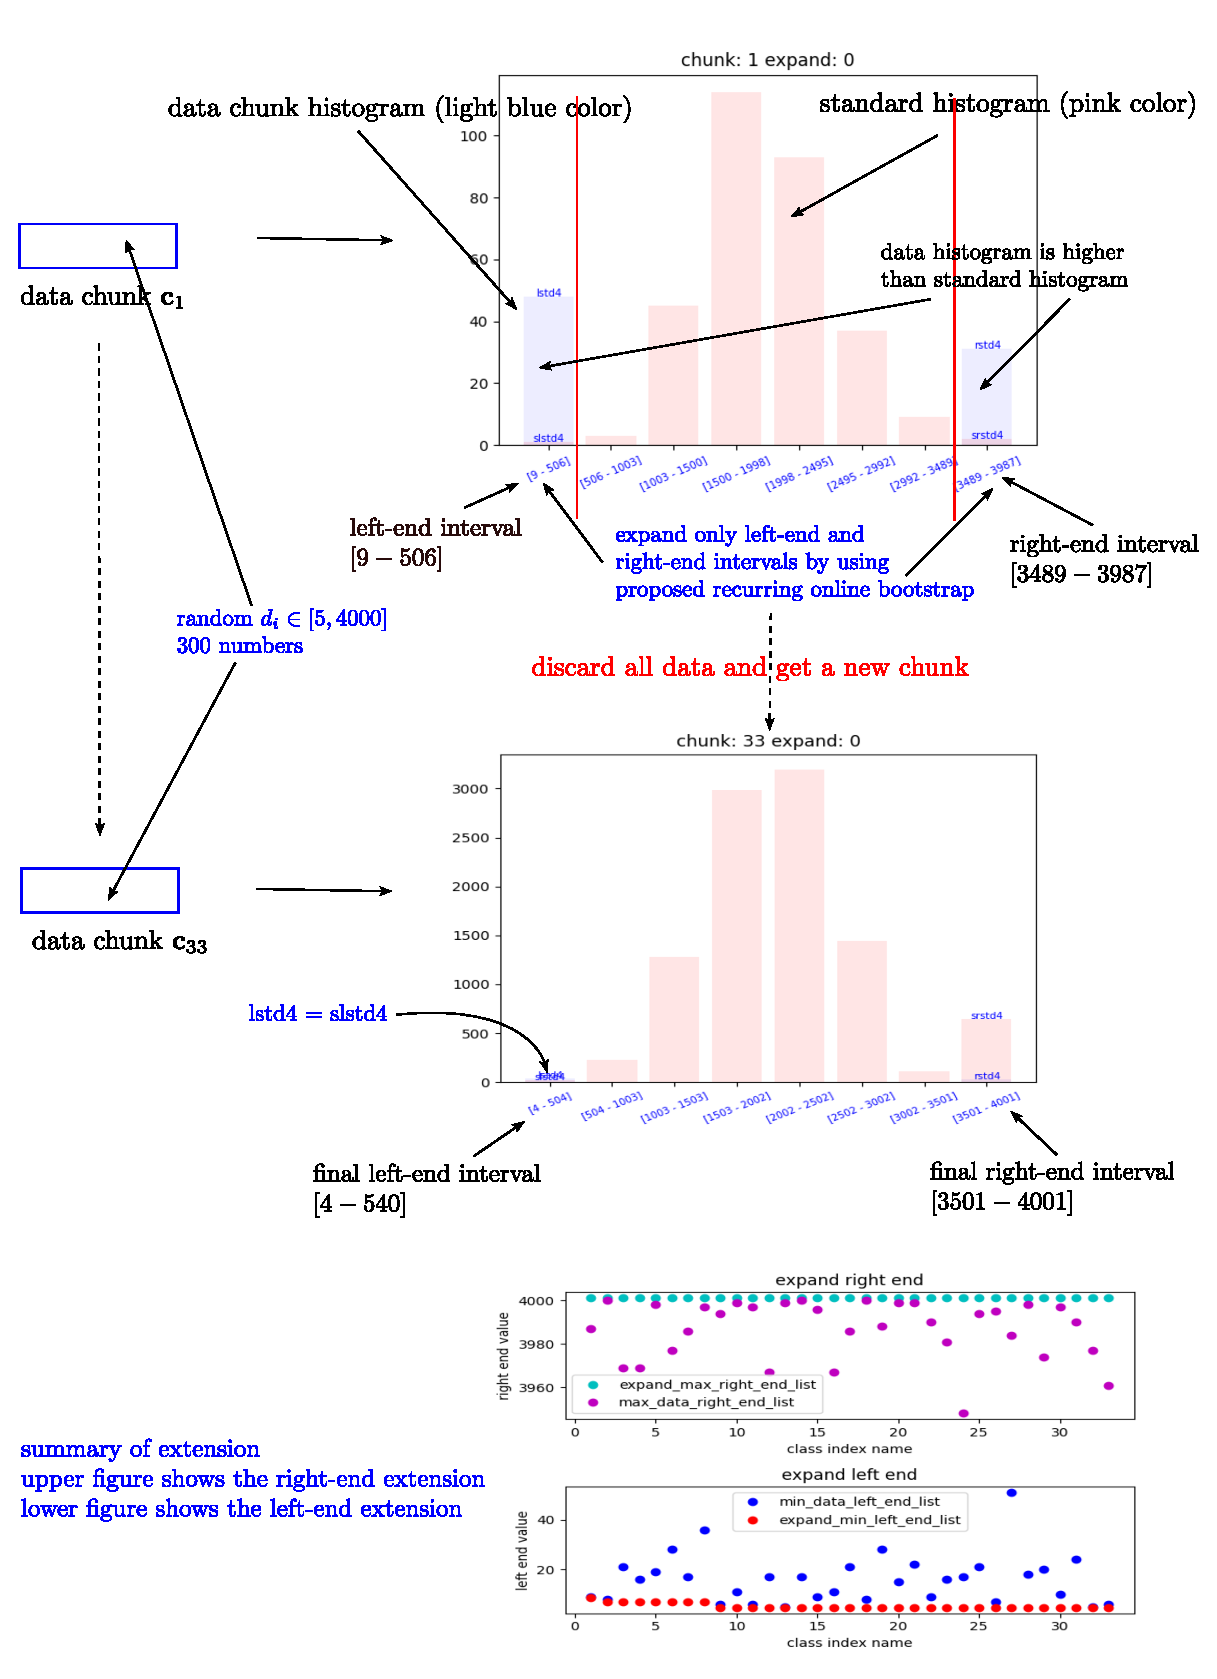
\includegraphics[scale = 0.6]{concept-framework.eps} 
\caption{Proposed concept of recurring online bootstrapping method.} 
\label{frame-work}
\end{figure*}

\section{RBULT Algorithms}
This section outlines the proposed algorithms for the recurring online bootstrap in a streaming 
environment, with or without outlier filtering. Suppose the data in $D$ are partitioned into eight equal 
intervals, $B = \{b_{1}, \ldots, b_{8}\}$. Let $L$ and $R$ be the left-end and right-end values  
%be the left-end value and $R$ be the right-end value
after bootstrapping at $b_{1}$ and $b_{8}$ respectively. Define $d^{(min)} = \min\limits_{d \in D}
(d)$ and $d^{(max)} = \max\limits_{d \in D}(d)$. There are four main algorithms:
\begin{enumerate}
\item Algorithm 1: Estimating the left-end and right-end values of $c_{1}$.
\item Algorithm 2: Estimating the left-end and right-end values of $c_{i}$ for $i > 1$.
\item Algorithm 3: Bootstrapping Data in %$h_{1}$ and $h_{8}$.
$b_{1}$ and $b_{8}$.
\item Algorithm 4: Eliminating outlier by z-score:
\end{enumerate}
The details of each algorithm are in the following subsections.

\subsection{Estimating the left-end and right-end values of $c_{1}$}
\vspace{0.2in}
\noindent
{\bf Algorithm 1:} Estimating left-end and right-end of $c_{1}$
\begin{tabbing}
\noindent
{\bf Input: } \= (1) First data chunk, %${\bf c}_{1}$.  \\
$c_{1}$.  \\
              \> (2) List $P$ of probability density functions. \\
              \> (3) \= Set of empty intervals $B =\{b_{1}, b_{2}, \ldots, b_{8}\}$ \\
              \>     \> and $|b_{i}|$ denotes the height.\\
              \> (4) Set of empty intervals $H=\{h_{1}, h_{2}, \ldots, h_{8}\}$ \\
              \>     \> and $|h_{i}|$ denotes the height.
\end{tabbing}
\begin{tabbing}
{\bf Output: } \= (1) Values of left end $L$ and right end $R$.\\
               \> (2) Set of intervals $B = \left\lbrace b_1,b_2,...,b_8 \right\rbrace $ %b_1,b_2,...,b_8 \right}$           
\end{tabbing}

\begin{tabbing}
1.~~ \= Load $c_{1}$ into $D$ and find the probabilistic \\
     \> distribution best fits the data in $D$ from list $P$ to \\
     \> create standard histogram $H$. \\
3.   \> Create 8-interval histogram $B$ from data in $D$. \\
4.   \> Find \= $d^{(min)}$ and $d^{(max)}$. \\
5.   \> {\bf While} $|b_{1}| > |h_{1}|$ {\bf or} $|b_{8}| > |h_{8}|$ {\bf do} \\
6.   \>        \> Bootstrap data in $b_{1}$ and $b_{8}$ to obtain $L$ and \\
     \>        \> $R$ by Algorithm 3. \\
7.   \>        \> Set mean $\mu = \frac{L + R}{2}$ and standard deviation \\
     \>        \> $\sigma = \frac{L - R}{8}$. \\
8.   \>        \> Include $L$ and $R$ into $D$. \\
9.   \>        \> Create histogram $H$ from data in $D$ by using \\
     \>        \> $\mu$ and $\sigma$ from step 7. \\
10.   \> {\bf EndWhile} \\
11.  \> Discard all data in $D$ except those in $b_{1}$ and $b_{8}$. \\
12.  \> Apply Algorithm 2 to next $c_{i}$ for $i > 1$.
\end{tabbing}

\subsection{Estimating left-end and right-end of $c_{i}$ for $i > 1$}
\vspace{0.2in}
\noindent
{\bf Algorithm 2:} Estimating left-end and right-end of $c_{i}$ for $i > 1$ %$i \geq 1$
\begin{tabbing}
{\bf Input: } \= (1) Data chunks, ${\bf c}_{i}$ for $i \geq 1$.  \\
              \> (2) \= Set of intervals $B =\{b_{1}, b_{2}, \ldots, b_{8}\}$. \\
              \>     \> from Algorithm 1. \\
              \> (3) $L$ and $R$ from Algorithm 1.
\end{tabbing}
\begin{tabbing}
{\bf Output: }\= Values of left end $L$ and right end $R$.          
\end{tabbing}
\begin{tabbing}
1.~~ \= {\bf While} \= there exists new incoming chunk $c_{i}$ {\bf do} \\
2.   \>             \> Load $c_{i}$ into $D$. \\
3.   \>             \> Eliminate outlier data from $D$ by Algorithm \\
     \>             \> 4. \\
4.   \>             \> Set $d^{(min)} = \min\limits_{d \in D}(d)$ and $d^{(max)} = 
                       \max\limits_{d \in D}(d)$. \\
5.   \>             \> {\bf If} $d^{(min)} < L$ {\bf then} Set $L = d^{(min)}$. \\
6.   \>             \> {\bf If} $d^{(max)} > R$ {\bf then} Set $R = d^{(max)}$. \\
7.   \>             \> Create histogram $B$ for data in $D$ from \\
     \>             \> mean $\mu = \frac{L + R}{2}$ and standard deviation \\
     \>             \> $\sigma = \frac{R - L}{8}$. \\
8.   \>             \> Create standard histogram $H$ of probabilistic \\
     \>             \> distribution found in Algorithm 1 with $\mu$ \\
     \>             \> and \= $\sigma$ from step 7. \\
9.   \>             \> {\bf While} $|b_{1}| > |h_{1}|$ {\bf or} $|b_{8}| > |h_{8}|$ {\bf do} \\
10.  \>             \>     \> Bootstrap data in $b_{1}$ and $b_{8}$ to obtain \\
     \>             \>     \> $L$ and $R$ by Algorithm 3. \\
11.  \>             \>     \> Set mean $\mu = \frac{L + R}{2}$ and standard \\
     \>             \>     \> deviation $\sigma = \frac{L - R}{8}$. \\
12.  \>             \>     \> Include $L$ and $R$ into $D$. \\
13.  \>             \>     \> Create histogram $B$ from data in $D$ \\
     \>             \>     \> using $\mu$ and $\sigma$ from step 11. \\
14.  \>             \> {\bf EndWhile} \\
15.  \>             \> Discard all data in $D$ except those in $b_{1}$\\
%     \>             \> and \hl{$b_{8}}$}. \\
16.  \> {\bf EndWhile}
\end{tabbing}

\subsection{Bootstrapping Data in $b_{1}$ and $b_{8}$}
\vspace{0.2in}
\noindent
{\bf Algorithm 3:} Bootstrapping Data in $b_{1}$ and $b_{8}$
\begin{tabbing}
{\bf Input: } \= (1) Data in $b_{1}$ and $b_{8}$. \\
              \> (2) Heights $|b_{1}|$ and $|b_{8}|$. \\
              \> (3) \= Predefined number of bootstrap samples \\
              \>     \> $N$. \\
              \> (4) Predefined number of bootstrap iterations \\
              \>     \> $M$.
\end{tabbing}
\begin{tabbing}
{\bf Output:} \= $L$ and $R$.
\end{tabbing}
\begin{tabbing}
1. ~~ \= Let $\mu_{h_{1}}$ be the mean of data in $h_{1}$ \\
2.   \> and $\mu_{h_{8}}$ be the mean of data in $h_{8}$. \\
%Let $\mu_{h_{1}}$ be the mean of data in $h_{1}$ and \\
%and $\mu_{h_{8}}$ be the mean of data in $h_{8}$.\\
--------------------- compute value of $L$ ---------------------\\

3.~~   \= Let $\mathcal{M} = \emptyset$ be a set of bootstrap means. \\
4.   \> Let $\mathcal{S} = \emptyset$ be a set of bootstrap standard deviations. \\
5.   \> {\bf For} \= $1 \leq i \leq M$ {\bf do} \\
6.   \>           \> Sample $N$ data in $b_{1}$ with replacement \\
     \>           \> and compute new mean $\hat{\mu}_{b_{1}}$. \\
7.   \>           \> Set $\mu_{b_{1}} = \frac{1}{2}(\hat{\mu}_{b_{1}} + \mu_{b_{1}}$). \\
8.   \>           \> Set $\mathcal{M} = \mathcal{M} \cup \{\mu_{b_{1}}\}$. \\
9.   \>           \> Sample $N$ data in $b_{1}$ with replacement \\
     \>           \> and compute new standard deviation $\hat{\sigma}_{b_{1}}$. \\
10.  \>           \> Set $\mathcal{S} = \mathcal{S} \cup \{\hat{\sigma}_{b_{1}}\}$. \\
11.  \> {\bf EndFor} \\
12.  \> Compute $\mu^{(boot)} = mean(\mathcal{M})$. \\
13.  \> Compute $\sigma^{(boot)} = mean(\mathcal{S})$. \\
14.  \> {\bf If} \= $mean(b_{1}) < \mu^{(boot)}$ {\bf then} \\
15.  \>          \> Set $L = \min(b_{1}) - |std(b_{1}) - \sigma^{(boot)}|$. \\
16.  \> {\bf If} \= $\mu^{(boot)} < mean(b_{1})$ {\bf then} \\
17.  \>          \> Set $L = \min(b_{1}) - |mean(b_{1}) - \mu^{(boot)}|$. \\
--------------------- compute value of $R$ -------------------- \\
18.  \> Let $\mathcal{M} = \emptyset$ be a set of bootstrap means. \\
19.  \> Let $\mathcal{S} = \emptyset$ be a set of bootstrap standard deviation. \\
20.  \> {\bf For} \= $1 \leq i \leq M$ {\bf do} \\
21.  \>           \> Sample $N$ data in $b_{8}$ with replacement \\
     \>           \> and compute new mean $\hat{\mu}_{b_{8}}$. \\
22.  \>           \> Set $\mu_{b_{8}} = \frac{1}{2}(\hat{\mu}_{b_{8}} + \mu_{b_{8}}$). \\
23.  \>           \> Set $\mathcal{M} = \mathcal{M} \cup \{\mu_{b_{8}}\}$. \\
24.  \>           \> Sample $N$ data in $b_{8}$ with replacement \\
     \>           \> and compute new standard deviation $\hat{\sigma}_{b_{8}}$. \\
25.  \>           \> Set $\mathcal{S} = \mathcal{S} \cup \{\hat{\sigma}_{b_{8}}\}$. \\
26.  \> {\bf EndFor} \\
27.  \> Compute $\mu^{(boot)} = mean(\mathcal{M})$. \\
28.  \> Compute $\sigma^{(boot)} = mean(\mathcal{S})$. \\
29.  \> {\bf If} \= $mean(b_{8}) < \mu^{(boot)}$ {\bf then} \\
30.  \>          \> Set $R = \max(b_{8}) + |std(b_{8}) - \sigma^{(boot)}|$. \\
31.  \> {\bf If} \= $\mu^{(boot)} < mean(b_{8})$ {\bf then} \\
32.  \>          \> Set $R = \max(b_{8}) + |mean(b_{
8}) - \mu^{(boot)}|$. 
\end{tabbing}
Define $mean(\mathcal{M})$ as a function to compute the average of data in a set $\mathcal{M}$. Also define $std(\mathcal{M})$ as a function to compute the standard deviation of data in a set $\mathcal{M}$, as well.  

\subsection{Eliminating Outlier Data}
\noindent
{\bf Algorithm 4:} Eliminating outlier by z-score:

\begin{tabbing}
{\bf Input:} \= (1) Data set $D$. \\
             \> (2) A constant $\tau$.
\end{tabbing}

\noindent
{\bf Output:} Data set $D$ without outliers.

\begin{tabbing}
1.~~ \= Compute mean $\mu$ of $D$. \\
2.   \> Compute standard deviation $\sigma$ of $D$. \\
3.   \> {\bf For} \= each $d \in D$ {\bf do} \\
4.   \>           \> Compute $z = \frac{|d - \mu|}{\sigma}$. \\
5.   \>           \> {\bf If} \= $z > \tau$ {\bf then} \\
6.   \>           \>          \> $D = D - \{d\}$. \\
7.   \> {\bf EndFor}
\end{tabbing}

\section{Theoretical Analysis}
The minimum and maximum numbers of expansion for the values of $L$ and $R$ can be theoretically analysed
in terms of probability as addressed in the following theorems. Suppose the size of population 
$\mathcal{P}$ is known to be $N$ and the size of each incoming chunk is $l$. Each datum has no duplicate. 
Let $p^{(min)} = \min(\mathcal{P})$ and $p^{(max)} = \max(\mathcal{P})$ be the the minimum and maximum 
data of the population $\mathcal{P}$, respectively.

\newtheorem{theorem}{Theorem}
\begin{theorem}
Assume that a chunk of $l$ data is picked one at a time without replacement from the population $\mathcal{P}$ with size $N$. 
The probability of having $p^{(min)}$ and $p^{(max)}$ in the first incoming chunk is 
$\frac{l(l-1)}{N(N-1)}$.

\begin{proof}
When $p^{(min)}$ and $p^{(max)}$ are in the first chunk, the rest of $l-2$ data must be randomly picked 
from $N-2$ data of population. The number of ways to pick $l-2$ data from $N-2$ data is
\begin{align*}
w = \left ( \begin{array}{c}
N-2 \\
l-2
\end{array}
\right )
\end{align*}
Each picked $l-2$ data with $p^{(min)}$ and $p^{(max)}$ can be combined with other $N-l$ data. There are
$(N-l)!$ possible permutations of $N-l$ data. Therefore, the total possible number of chunks $C$ having 
$p^{(min)}$ and $p^{(max)}$ is
\begin{align*}
c & = w \times (N-l)!  \\
  & = \left ( \begin{array}{c}
                 N-2 \\
                 l-2
                \end{array} 
                \right ) (N-l)!\\
  & = \frac{(N-2)!(N-l)!}{(l-2)!(N-2-l+2)!} \\
  & = \frac{(N-2)!}{(l-2)!} \\
\end{align*}
The total number of possible positions of $p^{(min)}$ and $p^{(max)}$ in the first chunk is $l!$. 
Therefore, all possible ways to have $p^{(min)}$ and $p^{(max)}$ in the first chunk is 
$\frac{l!(N-2)!}{(l-2)!} = l(l-1)(N-2)!$.
All possible sequences of data in the population is $N!$. Thus, the probability of having $p^{(min)}$ 
and $p^{(max)}$ in the first incoming chunk is $\frac{l(l-1)(N-2)!}{N!} = \frac{l(l-1)}{N(N-1)}$.  
\end{proof}
\end{theorem}

\begin{theorem}
Assume that a chunk of $l$ data is picked one at a time without replacement from population $\mathcal{P}$ with size $N$.
The probability of having $p^{(min)}$ and $p^{(max)}$ in the $i^{th}$ incoming chunk  for $i \geq 1$ is 
$\frac{l(l-1)}{N(N-1)}$.
\begin{proof}
%For $i>1$, the number of population is $N-l$. Without loss of generality, let $N-l=kl$. 
Let $S$ denote the sample space of events of generating $L$ data chunks from the observations in $\mathcal{P}$ by which $N=l\cdot L$.%, each data chunk  consisting of $l$ elements, sampled from a total of $N$ observations. 
The number of events in $S$ denoted by $|S|$, is the number of permutation of $N$ data divided by the permutation of $l$ elements of $L$ data chunks.  $|S|$ is mathematically expressed by

\begin{equation}
|S|=\frac{N!}{(l!)^L}. \label{eq:S}
\end{equation}
%$$|S|=\frac{N!}{(l!)^L}$$ 
Let $E_i\subset S$ denote the set of events where both $p^{(min)}$ and $p^{(max)}$ are contained within the $i^{th}$ data chunk. Applying the product rule of combinatorics, the total number of such events, denoted by $|E_i|$, is mathematically expressed as: 
\begin{equation}
%|E_i|=\binom{l}{2}\binom{N-2}{l-2}\frac{(N-l)!}{(l!)^{L-1}},\label{eq:E}
|E_i|=\binom{N-2}{l-2}\frac{(N-l)!}{(l!)^{L-1}},\label{eq:E}
\end{equation}
where $\binom{N-2}{k-2}$ represents the number of ways to select the remaining $l-2$ observations for the $i^{th}$ chunk from the $N-2$ available data (excluding $p^{(min)}$ and $p^{(max)}$)$, \frac{(N-l)!}{(l!)^{L-1}}$ denotes the number of ways to partition the remaining $N-l$ observations into the other $L-1$ data chunks, each of size $l$.

%\item[-] $\binom{l}{2}$ is the number of ways to pick the $p^{(min)}$ and $p^{(max)}$ in the $i^{th}$ chunk with size $l$,
%\item[-] $\binom{N-2}{k-2}$ represents the number of ways to select the remaining $l-2$ observations for the $i^{th}$ chunk from the $N-2$ available data (excluding $p^{(min)}$ and $p^{(max)}$), 
%\item[-] $\frac{(N-l)!}{(l!)^{L-1}}$ denotes the number of ways to partition the remaining $N-l$ observations into the other $L-1$ data chunks, each of size $l$.
%$$|E|=\binom{l}{2}\binom{N-2}{l-2}\frac{(N-l)!}{(l!)^{L-1}},$$

Based on Equations \ref{eq:S} and \ref{eq:E}, the probability of $p^{(min)}$ and $p^{(max)}$ being located within the $i^{th}$ incoming chunk, denoted by $P(E_i)$, is derived as follows:
\begin{align*}
    P(E_i) &= \frac{|E_i|}{|S|}    \notag\\
           &= \frac{\binom{N-2}{l-2}\frac{(N-l)!}{(l!)^{L-1}}}{\frac{N!}{(l!)^L}}\\
           &= \frac{\left(\frac{(N-2)!}{(l-2)!(N-l)!} \right)\left( \frac{(N-l)!}{(l!)^{L-1}}\right)}{\frac{N!}{(l!)^L}} \\
           &= \left(\frac{(N-2)!}{(l-2)!(N-l)!} \right)\left( \frac{(N-l)!}{(l!)^{L-1}}\right)\\
           &\left(\frac{l!(l!)^{L-1}}{N!}\right) \\
           &=\frac{(N-2)!(N-l)!l!(l!)^{L-1}}{(l-2)!(N-l)!(l!)^{L-1}N!},      \\
\end{align*}
finally, we obtain that
\begin{equation}
P(E_i) =\frac{l(l-1)}{N(N-1)}.
\end{equation}

Therefore, the probability of having $p^{(min)}$ and $p^{(max)}$ in the $i^{th}$ incoming chunk  for $i \geq 1$ is 
$\frac{l(l-1)}{N(N-1)}$.
%\begin{equation}
%P(E_i)  =\frac{l(l-1)}{N(N-1)}. \label{eq:PE}
%\end{equation}

%The result in Equation \ref{eq:PE} demonstrates that the inclusion of both $p^{(min)}$ and $p^{(max)}$ within a single chunk is governed by the ratio of the pairs available in a chunk to the total pairs in the entire dataset.


 
%is that (the number of ways to pick $p^{(min)}$ and $p^{(max)}$ in the $i{th}$ chunk) $\times$ 
%$$|S|=\frac{N!}{(l!)^L}$$ 
\end{proof} 
\end{theorem}

\newtheorem{corollary}{Corollary}

\begin{corollary}
Assuming that the joint occurrence of the minimum and maximum observations is restricted to a single chunk, the expected index of such a chunk is given by $E[X] = \frac{1}{2}\left(\frac{l(l-1)(L)(L+1)}{N(N-1)}\right)$ for the total number of $L$ data chunks.
\begin{proof}
Let $X \in \{1, 2, \dots, L\}$ be a discrete random variable representing the index of the chunk containing both $p^{(min)}$ and $p^{(max)}$. Given the assumption that this event must occur in exactly one of the $L$ chunks, and note that the probability is uniform across all chunks ($P(E_i) =\frac{l(l-1)}{N(N-1)}$ under this restriction), the expectation is calculated as follows:
\begin{align*}
E[X] &= \sum_{i=1}^{L} i \cdot P(X = i) \\
     &= \sum_{i=1}^{L} i \cdot \frac{l(l-1)}{N(N-1)} \\
     &= \left( \frac{L(L+1)}{2}\right)\left( \frac{l(l-1)}{N(N-1)}\right)\\
     &= \frac{1}{2}\left(\frac{l(l-1)(L)(L+1)}{N(N-1)}\right).
\end{align*}
%Applying the arithmetic series formula $\sum_{i=1}^{L} i = \frac{L(L+1)}{2}$, we obtain:
Finally, we obtain:
\begin{equation} 
E[X] = \frac{1}{2}\left(\frac{l(l-1)(L)(L+1)}{N(N-1)}\right) 
\end{equation}

\end{proof}
\end{corollary}


\section{Experiments}
\label{experiment}

% \subsection{Data for experiments}
\subsection{Experimental design}
This study comprehensively evaluates the range approximation method across two types 
of one-dimensional data populations: simulated data and real-world data. As detailed in Table 
\ref{tab:dist-params}, 
ten datasets were generated from five established statistical distributions, including $F$, $Chi-square$, 
$Normal$, $Wald$, and $Weibull$. Each has distinct parameter settings. For the $F$ distribution, %we implemented 
two configurations, $F(5, 10)$ and $F(5, 20)$, were considered to highlight  differences in their statistical 
characteristics. Although both distributions share the same numerator parameter, $\nu_1=5$, increasing the 
denominator parameter, $\nu_2$, from 10 to 20 results in notable changes in their properties. 
For the $Wald$ distribution, a smaller $\lambda$ value exhibits a more spread-out distribution 
with a range of $[0.0323, 15.1948]$. In contrast, a larger $\lambda$ value results in a more concentrated distribution around the mean, with a narrower range of $[0.1090, 12.8305]$.
For the $Normal$ distributions, we used the same mean of zero while varying the variances to 
$\sigma^2 = 1$ and $\sigma^2 = 16$, with ranges 
from $-3.6943$ to $4.2593$ and $-14.2604$ to $18.0044$, respectively. Both $Normal$ distributions share 
the same mean but have significantly different variances, 
allowing us to investigate the impact of different spread patterns under the same mean parameter, leading to distinct characteristics. For the $Chi-square$ 
distribution, $\chi^2(\nu=2)$ and $\chi^2(\nu=2)$ were simulated. The $\chi^2(\nu=2)$ distribution 
shows a highly right-skewed shape with its peak near zero and a range of $[0.0000, 21.9290]$, while $
\chi^2(\nu=10)$ displays a more symmetric shape, with a broader range of $[0.7468, 33.6357]$, reflecting greater spread and variability.
For the $Weibull$ distribution, $shape$ parameters of $1$ and $5$ were used to represent distinct behavioural characteristics.
%For the $Weibull$ distribution, different shape parameters of $1$ and $5$ \hl{were used to represent} 
%distinct \hl{behavioral} characteristics.
$Weibull$ with $shape=1$ behaves 
the same as an exponential distribution with a monotonically decreasing pattern and a wide range of 
[0.1090, 12.2323], characterised by a constant hazard rate, making it suitable for modelling 
random failures and exponential decay processes. In contrast, $Weibull$ with $shape=5$ presents a 
bell-shaped, nearly symmetric distribution with a narrower range of $[0.1209, 1.5980]$, 
featuring increasing failure rates over time and a more concentrated probability density. These significant differences in ranges and probability density 
distributions reflect their reliability engineering and failure analysis applications. In addition, 
we set the number of simulated data to 10,000 for all datasets, 
treating this as the population size for constructing the streaming data environment. The distributions of all experimental data for the entire population and for the random samples are 
illustrated in Figures \ref{case1:sim_pop}  - \ref{case1:sim_pop2}, using violin plots. The blue distribution represents the complete simulated population ($N=10,000$), while the red distribution represents a $30\%$ of random sample drawn from the population.

Additionally, we conducted more experiments on a sample dataset containing outliers. Outlier generation was achieved in two steps. First, the mean and standard deviation of the pre-defined population data were computed. Subsequently, a contamination rate ($0.05\%$ in this study) was used to determine the exact number of outliers to be added to the sample dataset.
%For outlier generation, we generated outlier data by first calculating the mean 
%and standard deviation of a pre-defined population data. Then, determines the number of outliers 
%to contaminate in the samples based on a specified contamination rate in this work  
%we set to $0.05\%$. 
Outliers were created by generating new values from a normal distribution at 
a significant distance from the original data mean, defined as a multiple of the standard deviation, set to 10 in this study. Specifically, half of the outliers were created on 
the left side (mean minus a multiple of the standard deviation). In contrast, the remaining were created on the 
right side (mean plus a multiple of the standard deviation). These newly generated outlier values were 
then combined with the sample data chunk to produce a new data chunk containing a specified proportion 
of outliers.

\begin{table}[htbp]
    \centering
    \caption{Description of statistical distribution's parameters, minimum and maximum values of the 
    simulation scenario.}
    \label{tab:dist-params}
    \begin{threeparttable}
    \begin{tabular}{cccc}
        \toprule
        \textbf{No.} & \textbf{Distribution} & \textbf{Minimum} & \textbf{Maximum} \\
        \midrule
        1 & $F(\nu_1 =5 ,\nu_2 =10)$ & 0.0083 & 52.4746 \\
        \midrule
         2 & $F(\nu_1 =5 ,\nu_2 =20)$ & 0.0219 & 127.5459 \\
         \midrule
         3 & $Wald(\mu =1.0 ,\lambda =0.5)$ & 0.0323 & 15.1948 \\
         \midrule
         4 & $Wald(\mu =1.0 ,\lambda =2.0)$ & 0.1090 & 12.8305 \\
         \midrule
         5 & $N(\mu =0.0 ,\sigma^2 =1.0)$ & -3.6943 & 4.2593 \\
         \midrule
         6 & $N(\mu =0.0 ,\sigma^2 =16.0)$ & -14.2604 & 18.0044 \\
         \midrule 
         7 & $\chi^2(\nu =2)$ & 0.0000 & 21.9290 \\
        \midrule
         8 & $\chi^2(\nu =10.0)$ & 0.7468 & 33.6357 \\
         \midrule
         9 & $Weibull(shape =1.0)$ & 0.1090 & 12.2323 \\
         \midrule
         10 & $Weibull(shape =5.0)$ & 0.1209 & 1.5980 \\
        \bottomrule
    \end{tabular}
    \begin{tablenotes}
          \scriptsize
          \item Note: The values in the Minimum and Maximum columns represent the population minimum and maximum values of the corresponding distribution.
    \end{tablenotes}
    \end{threeparttable}
\end{table}

\begin{figure*}[!t]
\centering
\begin{subfigure}[b]{0.4\textwidth}
    
\includegraphics[width=\textwidth,keepaspectratio]{fdistdfn5dfd10n10000.png}
    \caption{$F(\nu_1 =5 ,\nu_2 =10)$}
\end{subfigure}
\qquad
\begin{subfigure}[b]{0.4\textwidth}
    
\includegraphics[width=\textwidth,keepaspectratio]{fdistdfn5dfd20n10000.png}
    \caption{$F(\nu_1 =5 ,\nu_2 =20)$}
\end{subfigure}
\\
% \centering
\begin{subfigure}[b]{0.4\textwidth}
    
\includegraphics[width=\textwidth,keepaspectratio]{waldm1sd05n10000.png}
    \caption{$Wald(\mu =1.0 ,\lambda =0.5)$}
\end{subfigure}
\qquad
\begin{subfigure}[b]{0.4\textwidth}
    
\includegraphics[width=\textwidth,keepaspectratio]{waldm1sd2n10000.png}
    \caption{$Wald(\mu =1.0 ,\lambda =2.0)$}
\end{subfigure}
\caption{Simulated population and sample distribution for $F$ and $Wald$ distributions with $N=10,000$}
\label{case1:sim_pop} 
\vspace{0.5em} % Adds a small vertical space
\scriptsize % Changes the font size to footnotesize
Note: The blue violin plots shows the distribution of the complete simulated population ($N=10,000$), while the red one shows the distribution of $30\%$ of random sample drawn from the population
\end{figure*}

\begin{figure*}[!t]
\centering
\begin{subfigure}[b]{0.4\textwidth}
    
\includegraphics[width=\textwidth,keepaspectratio]{normalm0sd1n10000.png}
    \caption{$N(\mu =0 ,\sigma^2 =1)$}
\end{subfigure}
\qquad
\begin{subfigure}[b]{0.4\textwidth}
    
\includegraphics[width=\textwidth,keepaspectratio]{normalm0sd4n10000.png}
    \caption{$N(\mu =0 ,\sigma^2 =16)$}
\end{subfigure}
\\
\begin{subfigure}[b]{0.4\textwidth}
    
\includegraphics[width=\textwidth,keepaspectratio]{chi2df2n10000.png}
    \caption{$\chi^2(\nu =2)$}
\end{subfigure}
\qquad
\begin{subfigure}[b]{0.4\textwidth}
    
\includegraphics[width=\textwidth,keepaspectratio]{chi2df10n10000.png}
    \caption{$\chi^2(\nu =10)$}
\end{subfigure}
\\
\begin{subfigure}[b]{0.4\textwidth}
    
\includegraphics[width=\textwidth,keepaspectratio]{wiebullshape1n10000.png}
    \caption{$Weibull(shape = 1.0)$}
\end{subfigure}
\qquad
\begin{subfigure}[b]{0.4\textwidth}
    
\includegraphics[width=\textwidth,keepaspectratio]{wiebullshape5n10000.png}
    \caption{$Weibull(shape = 5.0)$}
\end{subfigure}
\caption{Simulated population and sample distribution for $Normal$, $\chi^2$, and $Weibull$ distributions 
with $N=10,000$}\label{case1:sim_pop2} 
\vspace{0.5em} % Adds a small vertical space
\scriptsize % Changes the font size to footnotesize
Note: The blue violin plots shows the distribution of the complete simulated population ($N=10,000$), while the red one shows the distribution of $30\%$ of random sample drawn from the population
\end{figure*}

\begin{figure*}[!t]
\centering
\begin{subfigure}[b]{0.4\textwidth}
    
\includegraphics[width=\textwidth,keepaspectratio]{laptop_prices.png}
    \caption{Labtop prices}
\end{subfigure}
\qquad
\begin{subfigure}[b]{0.4\textwidth}
    
\includegraphics[width=\textwidth,keepaspectratio]{Electronic_sales_Sep2023-Sep2024.png}
    \caption{Electronic sales}
\end{subfigure}
\\
\begin{subfigure}[b]{0.4\textwidth}
    
\includegraphics[width=\textwidth,keepaspectratio]{Ecommerce_Sales_Prediction_Dataset.png}
    \caption{E-commerce sales}
\end{subfigure}
\qquad
\begin{subfigure}[b]{0.4\textwidth}
    
\includegraphics[width=\textwidth,keepaspectratio]{world_tourism_economy_data.png}
    \caption{World tourism economy}
\end{subfigure}

% \subfigure[Labtop prices]{%%\label{}%
%     
\includegraphics[scale = 0.3]{laptop_prices.png}
% }
% \qquad
% \subfigure[Electronic sales]{%%\label{}%
%     
\includegraphics[scale = 0.3]{Electronic_sales_Sep2023-Sep2024.png}
% }
% \\
% \subfigure[E-commerce sales]{%%\label{}%
%     
\includegraphics[scale = 0.3]{Ecommerce_Sales_Prediction_Dataset.png}
% }
% \qquad
% \subfigure[World tourism economy]{%%\label{}%
%     
\includegraphics[scale = 0.3]{world_tourism_economy_data.png}
% }

\caption{Real-world population data distribution for laptop prices, electronic sales, e-commerce sales, 
and world tourism economy.}\label{realworld} 
\vspace{0.5em} % Adds a small vertical space
\scriptsize % Changes the font size to footnotesize
Note: The blue violin plots shows the distribution of the complete simulated population ($N=10,000$), while the red one shows the distribution of $30\%$ of random sample drawn from the population
\end{figure*}

In our experiments on real-world scenarios, we examined four datasets representing various 
economic sectors, as summarised in Table  \ref{tab:real-params}. These datasets were selected to 
evaluate the proposed methodology across different real-world applications and value distributions. The first dataset is 
the laptop prices in $Euros$ \cite{realworld:laptop}, with values ranging from 174.00 to 6,099.00. This 
dataset comprehensively represents price distribution in the technology retail sector. The second dataset 
is electronic sales transactions\cite{realworld:elec_sales}, with values ranging from
20.75 to 11, 396.80. This extensive range captures the full spectrum of electronic retail activity, from 
minor accessory purchases to significant investments in premium electronic equipment. The third dataset 
examines e-commerce sales data \cite{realworld:ecom}, with transaction values ranging from
100.30 to 9, 995.62. This range reflects the diverse nature of online retail transactions in the digital 
marketplace. The distribution of the dataset provides valuable insights into e-commerce transaction 
patterns and consumer spending behaviours. The fourth dataset is the tourism and economic impact dataset 
\cite{realworld:tourism}, which uses tourism expenditures in $U.S.$ dollars. The range of this 
variable is from 0.1578 to 28.1923. This dataset's scale and distribution characteristics offer an 
important perspective on the applicability of the proposed
 methodology to macroeconomic indicators. The 
histograms of the real-world datasets are shown in Figure \ref{realworld}.

\begin{table}[htbp]
    \centering
    \caption{Description of minimum and maximum values of the real-world scenario.}
    \label{tab:real-params}
    \begin{threeparttable}
    \begin{tabular}{cccc}
        \toprule
        \textbf{No.} & \textbf{Dataset} & \textbf{Minimum} & \textbf{Maximum} \\
        \midrule
        1 & Laptop prices & 174.00 & 6,099.00 \\
        \midrule
         2 & Electronic sales & 20.75 & 11,396.80 \\
         \midrule
         3 & E-commerce sales & 100.30 & 9,995.62 \\
         \midrule
         4 & World tourism economy & 0.1578 & 28.1923 \\
        \bottomrule
    \end{tabular}
    \begin{tablenotes}
          \scriptsize
          \item Note: The values in the Minimum and Maximum columns represent the population minimum and maximum values of the corresponding dataset.
    \end{tablenotes}
    \end{threeparttable}
\end{table}

\subsection{Experimental results}
In this study, we established a streaming data chunk environment to evaluate 
our proposed methods. Given a population $\mathcal{P}$ with a range of $[L_{\mathcal{P}},R_{\mathcal{P}}]$, we randomly selected a set of samples ${\bf X} = \left\{x_i \in \mathcal{P}|\,\,{\rm for}\,
\,i=1,2,\ldots,n\,\,{\rm and}\,\, n<N\right\}$ from the population. These samples were used to create 
streaming data chunks ${\bf c}_i$. We empirically examined three bootstrapping-based methods for 
range approximation. The first method, method $a$, implements the proposed algorithms without noise 
filtering for the bootstrapping-based range approximation. The second method, method $b$ referred to as double 
online bootstrap, extends method $a$ by approximating the minimum and maximum of boostrapping datasets by performing the 
bootstrapping procedures detailed in Algorithms 2 and 3. The third method, method $c$, 
represents the traditional bootstrapping approach where data from streaming chunks are accumulated before performing 
bootstrapping. The method $d$ is the online bootstrap with noise filtering. To evaluate the 
performance of these methods, we employed the range error, which quantifies the accuracy of the range approximation. The range error is calculated as follows:

%For creating the streaming data chunks environment, given a population $\mathbb{P}$ with a range of $[l^{(min)},r^{(max)}]$ and size $N$, let ${\bf X} = \left\{x_i \in \mathbb{P}|\,\,{\rm for}\,\,i=1,2,\ldots,n\,\,{\rm and}\,\, n<N\right\}$ be the set of samples randomly selected from the population $\mathbb{P}$. The sample set ${\bf X}$ was applied to create a streaming data chunk with size $L$. In this work, three bootrapping-based methods were empirically examined. The first method, $online1Bt$, is the bootstrapping-based method referring to the proposed algorithms. The second one, $online2Bt$, is extended from the $online1Bt$ by which $min(b1)$ and $max(b2)$ in steps 18 and 21 in Algorithms 3 and 4 are replaced by the bootstrapping expansion of Algorithms 2.1 and 2.2, respectively. The third one, $AccBt$, is the traditional bootstrapping method in which the data in the streaming data chunk are accumulated for bootstrapping. Two measures were computed for the performance evaluation: the range error and the number of samples for the bootstrapping computation. The range error is calculated as follows: 

$$rage\_error = pop\_range-est\_range,$$

where $pop\_range = R_{\mathcal{P}}-L_{\mathcal{P}}$, denotes the population range, and $est\_range = R-L$ denotes the estimated range.

\subsubsection{Results on the streaming environment from simulated data scenario}

The experimental results of four methods for range approximation with the equally pre-defined chunk sizes of $|\mathbf{c}_i|=50$ and 
$|\mathbf{c}_i|=500$ for simulated data without noise are given in Tables \ref{tab:res-siml50nonoise} and 
\ref{tab:res_sim500nonoise}. The methods are: Online Bootstrap ($a$), Double Online Bootstrap ($b$), 
Traditional Bootstrap ($c$), and Online Bootstrap with outlier filtering ($d$). A key metric for 
evaluating these methods is the Range error, which measures the difference between the estimated 
range and the true population range. A smaller range error indicates better performance. The results in Tables \ref{tab:res-siml50nonoise} 
show that the proposed online bootstrap methods ($a, b, d$) are more effective at approximating 
the population range than the traditional bootstrap method ($c$) in a streaming data environment. 
The best performance is typically observed with the online bootstrap approach that incorporates outlier elimination ($d$), as it %is better able to handle 
more effectively handles streaming data and yields a more accurate range 
estimate. 

For comparison on online bootstrap methods, the Online Bootstrap ($a$) and the Online Bootstrap 
with outlier elimination ($d$) %perform comparably. 
exhibit comparable performance; however, the method with outlier elimination often has a slight edge 
in accuracy, as reflected by its marginally lower range error in most cases. 
The Double Online Bootstrap ($b$) also performs competitively but does not consistently outperform the single 
online bootstrap methods. To further assess statistical significance, paired Student t-tests or Wilcoxon signed-rank tests were used to 
compare the performance of the Online Bootstrap with outlier elimination ($d$) with that of the other three methods 
across all datasets. The null hypothesis was given as follows: $H_0$: "{\it There is no significant 
difference in the range error mean between Method d and the compared method}" while the alternative hypothesis was, 
$H_1$: "{\it There is a significant difference in range error mean 
between method d and the compared method}" The results show that, for the majority
of the datasets, the $H_0$ is rejected, indicating that method $d$ provides a statistically  
%of the datasets, the $H_0$​ is rejected, indicating that Method d provides a statistically 
significant improvement in range approximation compared to the other methods, particularly 
the traditional bootstrap method. For Table \ref{tab:res_sim500nonoise}, across all datasets, 
the online bootstrap methods ($a, b$, and $d$) consistently outperform the Traditional Bootstrap ($c$). 
For instance, in the $F(5,10)$ distribution, the traditional bootstrap's range error is $26.40$, 
while the online bootstrap methods maintain a substantially lower error of $24.17$. Notably, the Online Bootstrap 
with outlier elimination ($d$) most frequently  achieves the lowest range 
error, particularly for the $F$, $Chi-square$, and $Weibull$ distributions, where it 
provides the most precise range estimates.

\begin{table*}[h!]    
\centering
\caption{Estimated results for a chunk size $|{\bf c}|=50$ in simulated datasets without noise.}
\label{tab:res-siml50nonoise}
\begin{threeparttable}
\begin{tabular}{|c|c|c|c|c|c|}
\hline
\multirow{2}{*}{No.} & \multirow{2}{*}{Distribution} & Population range & 
Estimated range&Range error& \multirow{2}{*}{\it{Reject} $H_0$} \\
&&$(pop\_range)$&$(est\_range)$&$(rage\_error)$& \\
\hline
\multirow{4}{*}{1.} & \multirow{4}{*}{$F(5 ,10)$}&\multirow{4}{*}{[0.0083, 52.47]} & $[0.0066, 28.30]_{a}$& 
    \bf{24.17} &False$_t$\\
&&&$[0.0067, 28.30]_{b}$ & \bf{24.17} & True$_t$\\
&&&$[0.0092, 26.07]_c$ & 26.40  & True$_t$\\
&&&$[0.0067, 28.30]_{d}$ &  \bf{24.17} & - \\
\hline
\multirow{4}{*}{2.} & \multirow{4}{*}{$F(5 ,20)$}&\multirow{4}{*}{[0.0219, 127.55]} & $[0.0374, 39.56]_a$& 
    \bf{88.00} & False$_t$\\
    &&&$[0.0374, 39.56]_b$ & \bf{88.00} & True$_t$\\
    &&&$[0.0404, 37.23]_c$ & 90.35 & True$_t$\\
    &&&$[0.0374, 39.56]_d$ &  \bf{88.00} & - \\
\hline
\multirow{4}{*}{3.} & \multirow{4}{*}{$Wald(1.0 ,0.5)$}&\multirow{4}{*}{[0.0323, 15.19]} & 
$[0.0355, 15.10]_a$& 
    \bf{0.09} & False$_t$\\
    &&&$[0.0414, 15.10]_b$ & 0.10 & True$_t$\\
    &&&$[0.0415, 14.59]_c$ & 0.61 & False$_t$\\
    &&&$[0.0344, 15.10]_d$ & \bf{0.09} & - \\

\hline
\multirow{4}{*}{4.} & \multirow{4}{*}{$Wald(1.0 ,2.0)$}&\multirow{4}{*}{[0.1090, 12.83]} & 
$[0.1279, 6.47]_a$& 
    \bf{6.38} & False$_w$\\
    &&&$[0.1280, 6.47]_b$ & \bf{6.38} & False$_w$\\
    &&&$[0.1298, 5.86]_c$ & 6.99      &  False$_w$\\
    &&&$[0.1254, 6.47]_d$ & \bf{6.38} &  - \\    
\hline
\multirow{4}{*}{5.} & \multirow{4}{*}{$N(0 ,1)$}&\multirow{4}{*}{[-3.6943, 4.26]} & $[-3.6943, 3.93]_a$& 
    \bf{0.33} & False$_t$\\
    &&&$[-3.6943, 3.93]_b$ & \bf{0.33} & False$_t$\\
    &&&$[-3.4916, 3.69]_c$ & 0.77      & True$_t$\\
    &&&$[-3.6943, 3.93]_a$ & \bf{0.33} &  - \\    

\hline
\multirow{4}{*}{6.} & \multirow{4}{*}{$N(0 ,4)$}&\multirow{4}{*}{[-14.26, 18.00]} & $[-13.93, 18.00]_a$& 
    \bf{0.33} & False$_t$\\
    &&&$[-13.93, 18.00]_b$ & \bf{0.33} & False$_t$\\
    &&&$[-13.71, 16.74]_c$ & 1.81      & True$_t$\\
    &&&$[-13.93, 18.00]_d$ & \bf{0.33} & - \\    

\hline
\multirow{4}{*}{7.} & \multirow{4}{*}{$\chi^2(10)$}&\multirow{4}{*}{[0.7468, 33.64]} & [$1.0809, 30.55]_a$& 
    \bf{3.42} & False$_t$\\
    &&&$[1.0809, 30.55]_b$ & \bf{3.42} & False$_t$\\
    &&&$[1.2533, 29.95]_c$ & 4.19      & False$_t$\\
    &&&$[1.0809, 30.55]_d$ & \bf{3.42} &  - \\    

\hline
\multirow{4}{*}{8.} & \multirow{4}{*}{$\chi^2(2)$}&\multirow{4}{*}{[0.0000, 21.93]} & $[-0.0008, 17.10]_a$& 
    \bf{4.82} & True$_t$\\
    &&&$[0.0001, 17.10]_b$ & \bf{4.82} & True$_t$\\
    &&&$[0.0002, 16.18]_c$ & 5.75      & True$_t$\\
    &&&$[-0.0057, 17.10]_d$ & \bf{4.82} & - \\       
    
\hline
\multirow{4}{*}{9.} & \multirow{4}{*}{$Weibull(1)$}&\multirow{4}{*}{[0.0000, 12.23]} & $[-0.0010, 12.23]_a$& 
    \bf{-0.00} & False$_t$\\
    &&&$[0.0001, 12.23]_b$ & \bf{0.00} & True$_t$\\
    &&&$[0.0002, 10.47]_c$ & 1.77      & False$_t$\\
    &&&$[-0.0087, 12.23]_d$ & -0.01 & - \\  
\hline
\multirow{4}{*}{10.} & \multirow{4}{*}{$Weibull(5)$}&\multirow{4}{*}{[0.1209, 1.60]} & $[0.1812, 1.56]_a$& 
    \bf{0.10} & False$_t$\\
    &&&$[0.1812, 1.56]_b$ & \bf{0.10} & False$_t$\\
    &&&$[0.1988, 1.55]_c$ & 0.12      & Flase$_t$\\
    &&&$[0.1812, 1.56]_d$ & \bf{0.10} & - \\    
\bottomrule
\end{tabular}
\begin{tablenotes}
          \scriptsize
          \item - Estimated range with the subscripts a, b, and d stand for online bootstrap, double online bootstrap, traditional bootstrap, and online bootstrap with noise filtering estimators, respectively.
          \item - Range error, indicated by the bold typeface, shows the minimum error. Its positive or negative values suggest whether the estimated range is narrower or wider than the true population range, respectively.
         \item - Hypothesis test: $H_0:$ "There is no significant difference in the mean range error between Method d and 
         the compared method over the specified time period.
    \end{tablenotes}
\end{threeparttable}
\end{table*}

\begin{table*}[h!]
\centering
\caption{Estimated results for a chunk size $|{\bf c}|=500$ in simulated datasets.}
\label{tab:res_sim500nonoise}
\begin{threeparttable}
\begin{tabular}{|c|c|c|c|c|c|}
\hline
\multirow{2}{*}{No.} & \multirow{2}{*}{Distribution} & Population range & 
Estimated range&Range error& \multirow{2}{*}{\it{Reject} $H_0$} \\
&&$(pop\_range)$&$(est\_range)$&$(rage\_error)$& \\
\hline
\multirow{4}{*}{1.} & \multirow{4}{*}{$F(5 ,10)$}&\multirow{4}{*}{[0.0083, 52.47]} & $[0.0066, 28.30]_a$& 
    \bf{24.17} & False$_t$\\
&&&$[0.0067, 28.30]_b$ & \bf{24.17} & True$_t$\\
&&&$[0.0092, 26.07]_c$ & 26.40 & True$_t$\\
&&&$[0.0067, 28.30]_d$ & \bf{24.17} & - \\
\hline
\multirow{4}{*}{2.} & \multirow{4}{*}{$F(5 ,20)$}&\multirow{4}{*}{[0.0219, 127.55]} & $[0.0374, 39.56]_a$& 
    \bf{88.00} & False$_t$\\
&&&$[0.0368, 15.10]_b$ & \bf{88.00} &  True$_t$\\
&&&$[0.0404, 37.54]_c$ & 90.03 &  True$_t$\\
&&&$[0.0374, 39.56]_d$ & \bf{88.00} &  - \\
\hline
\multirow{4}{*}{3.} & \multirow{4}{*}{$Wald(1.0 ,0.5)$}&\multirow{4}{*}{[0.0323, 15.19]} & 
$[0.0368, 15.10]_a$& 
    \bf{0.10} &False$_w$\\
    &&&$[0.0368, 15.10]_b$ & \bf{0.10} & False$_w$\\
    &&&$[0.0384, 14.62]_c$ & 0.58 & False$_w$\\
    &&&$[0.0364, 15.10]_d$ & \bf{0.10} & - \\
\hline
\multirow{4}{*}{4.} & \multirow{4}{*}{$Wald(1.0 ,2.0)$}&\multirow{4}{*}{[0.1090, 12.83]} & 
$[0.1270, 6.47]_a$& 
    \bf{6.38} & False$_w$\\
    &&&$[0.1810, 6.47]_b$ & 6.43      & True$_w$\\
    &&&$[0.1298, 5.88]_c$ & 6.99      & False$_w$\\
    &&&$[0.1273, 6.47]_d$ & \bf{6.38} & - \\
\hline
\multirow{4}{*}{5.} & \multirow{4}{*}{$N(0 ,1)$}&\multirow{4}{*}{[-3.6943, 4.26]} & $[-3.6943, 3.93]_a$& 
    \bf{0.33} & True$_t$\\
    &&&$[-3.6943, 3.93]_b$ & \bf{0.33} & True$_t$\\
    &&&$[-3.5066, 3.69]_c$ & 0.76      & True$_t$\\
    &&&$[-3.6943, 3.93]_d$ & \bf{0.33} & - \\    
\hline
\multirow{4}{*}{6.} & \multirow{4}{*}{$N(0 ,4)$}&\multirow{4}{*}{[-14.26, 18.00]} & $[-13.93, 18.00]_a$& 
    \bf{0.33} & False$_t$\\
    &&&$[-13.93, 18.00]_b$ & \bf{0.33} & False$_t$\\
    &&&$[-13.71, 16.94]_c$ & 1.64      & True$_t$\\
    &&&$[-13.93, 18.00]_d$ & \bf{0.33} & - \\
\hline
\multirow{4}{*}{7.} & \multirow{4}{*}{$\chi^2(2)$}&\multirow{4}{*}{[0.7468, 33.64]} & $[1.0809, 30.55]_a$& 
    \bf{3.42} & False$_w$\\
    &&&$[1.0809, 30.55]_b$ & \bf{3.42} & False$_w$\\
    &&&$[1.2471, 29.92]_c$ & 4.21      & False$_w$\\
    &&&$[1.0809, 30.55]_d$ & \bf{3.42} & - \\                
\hline
\multirow{4}{*}{8.} & \multirow{4}{*}{$\chi^2(10)$}&\multirow{4}{*}{[0.0000, 21.93]} & $[0.0001, 17.10]_a$& 
    \bf{4.83} & False$_w$\\
    &&&$[0.0001, 17.10]_b$ & \bf{4.83} & True$_t$\\
    &&&$[0.0002, 16.18]_c$ & 5.75      & False$_w$\\
    &&&$[-0.0003, 17.10]_d$ & \bf{4.82} & - \\
\hline
\multirow{4}{*}{9.} & \multirow{4}{*}{$Weibull(1)$}&\multirow{4}{*}{[0.0000, 12.23]} & 
$[-0.0025, 12.23]_a$& 
    \bf{-0.00} & False$_w$\\
    &&&$[0.0021, 12.23]_b$ & \bf{0.00} & True$_t$\\
    &&&$[0.0002, 10.47]_c$ & 1.76      & Flase$_w$\\
    &&&$[0.0001, 12.23]_d$ & \bf{0.00} & - \\
\hline
\multirow{4}{*}{10.} & \multirow{4}{*}{$Weibull(5)$}&\multirow{4}{*}{[0.1209, 1.60]} & $[0.1812, 1.56]_a$& 
    \bf{0.10} & False$_t$\\
    &&&$[0.2351, 1.47]_b$ & 0.25 & True$_w$\\
    &&&$[0.2002, 1.55]_c$ & 0.12      & True$_w$\\
    &&&$[0.1812, 1.56]_d$ & \bf{0.10} & - \\    
  
\bottomrule
\end{tabular}
\begin{tablenotes}
          \scriptsize
          \item - Estimated range with the subscripts SaS, SbS, and SdS stand for online bootstrap, double online bootstrap, traditional bootstrap, and online bootstrap with noise filtering estimators, respectively.
          \item - Range error, indicated by the bold typeface, shows the minimum error. Its positive or negative values indicate whether the estimated range is narrower or wider than the true population range, respectively.
         \item - Hypothesis test: $H_0:$ "There is no significant difference in the range error mean between method $d$ and 
         the compared method over the specified time period.
    \end{tablenotes}
\end{threeparttable}
\end{table*}

\subsubsection{Results on the streaming environment from simulated data with an outlier contaminating scenario}



Table \ref{tab:res_sim50_noise} displays the performance of four methods for 
range approximation with the chunk size of $|{\bf c}_i|=50$, when the simulated data is mixed with noise. 
The results highlight a significant difference in how the methods handle data contamination. 
Methods $a$ and $b$ (Online Bootstrap and Double Online Bootstrap) frequently fail to produce 
 valid range approximations for non-negative distributions (e.g., the $F$ and $\chi^2$) distributions.
This failure is indicated by "$n/a$" in the Range error, 
as the estimated range becomes negative and the error cannot be computed. The traditional bootstrap (method $c$) also fails to 
produce valid results for these distributions. In contrast, the Online Bootstrap with Outlier Filtering 
(method $d$) consistently provides valid and accurate range estimates, even for the most challenging 
non-negative distributions. For example, in the $F(5,10)$ and $F(5,20)$ distributions, method $d$ 
provides  low range errors of 0.02 and 77.20, respectively, while the other methods are unable to 
compute valid errors. For distributions where all methods yield valid estimates (e.g., Wald and Weibull distributions), 
the online methods ($a, b, d$) generally have smaller range errors than the traditional method ($c$). 
The Online Bootstrap with Outlier Filtering ($d$) often achieves the lowest error, with range errors 
of $0.10$ for the $Wald(1.0, 0.5)$ distribution and $0.00$ for the $Weibull(1)$ distribution.

For Table \ref{tab:res_sim500_noise}, the methods $a$ (Online Bootstrap), $b$ (Double Online Bootstrap), 
and $c$ (Traditional Bootstrap) frequently fail to provide a valid range approximation for distributions 
with a non-negative population range, such as the $F$ and $\chi^2$ distributions. In these cases, the 
estimated range includes negative values, making the error calculation invalid, which highlights the 
lack of robustness in a noisy, streaming environment. In contrast, the Online Bootstrap with Outlier Filtering 
(Method $d$). % is the most robust and accurate method. 
It consistently provides valid range estimates for all distributions. For challenging non-negative 
distributions, it yields very low range errors, such as 77.20 for the $F(5,20)$ distribution, while 
other methods fail. For distributions where all methods produce valid results (e.g., $Wald$ and $Weibull$), 
the online methods generally outperform the traditional method. 
The outlier-filtered approach (Method $d$) often achieves the lowest range error.

\begin{table*}[h!]
\centering
\caption{Estimated results for chunk size $|{\bf c}|=50$ with mixing outlier data in simulated datasets.}
\label{tab:res_sim50_noise}
\begin{threeparttable}
\begin{tabular}{|c|c|c|c|c|c|}
\hline
\multirow{2}{*}{No.} & \multirow{2}{*}{Distribution} & Population range & 
Estimated range&Range error& \multirow{2}{*}{\it{Reject} $H_0$} \\
&&$(pop\_range)$&$(est\_range)$&$(rage\_error)$& \\
\hline
\multirow{4}{*}{1.} & \multirow{4}{*}{$F(5 ,10)$}&\multirow{4}{*}{[0.0083, 52.47]} & $[-22.66, 52.47]_a$& 
    $n/a$ & $n/a$\\
&&&$[0.0800, 52.47]_b$ & 0.07 & True$_t$\\
&&&$[-19.44, 44.62]_c$ & $n/a$ & $n/a$\\
&&&$[0.0290, 52.47]_d$ & \bf{0.02} & - \\
\hline
\multirow{4}{*}{2.} & \multirow{4}{*}{$F(5 ,20)$}&\multirow{4}{*}{[0.0219, 127.55]} & $[-20.66, 50.35]_a$& 
    $n/a$ & $n/a$\\
    &&&$[0.0232, 50.35]_b$ & 77.20 & True$_t$\\
    &&&$[-22.99, 43.23]_c$ & $n/a$ & $n/a$ \\
    &&&$[0.0219, 50.35]_d$ & 77.20 & -  \\
\hline
\multirow{4}{*}{3.} & \multirow{4}{*}{$Wald(1.0 ,0.5)$}&\multirow{4}{*}{[0.0323, 15.19]} & 
$[-13.17, 15.10]_a$& 
    $n/a$ & $n/a$\\
    &&&$[0.0400, 15.10]_b$ & \bf{0.10} & True$_t$\\
    &&&$[-11.73, 14.89]_c$ & $n/a$ & $n/a$\\
    &&&$[0.0363, 15.10]_d$ & \bf{0.10} &- \\

\hline
\multirow{4}{*}{4.} & \multirow{4}{*}{$Wald(1.0 ,2.0)$}&\multirow{4}{*}{[0.1090, 12.83]} & 
$[-6.25, 8.76]_a$& 
     $n/a$ & $n/a$ \\
    &&&$[0.1280, 8.76]_b$ & -13.11 & -\\
    &&&$[-5.28, 8.50]_c$ & $n/a$ & $n/a$\\
    &&&$[-5.92, 8.76]_d$& $n/a$ & $n/a$\\    
\hline
\multirow{4}{*}{5.} & \multirow{4}{*}{$N(0 ,1)$}&\multirow{4}{*}{[-3.6943, 4.26]} & $[-9.97, 10.16]_a$& 
    -12.17 & False$_t$\\
    &&&$[-9.97, 10.16]_b$ & -12.17 & False$_t$\\
    &&&$[-8.83, 9.16]_c$ & \bf{-10.67}      &True$_t$\\
    &&&$[-9.97, 10.16]_d$ & -12.17 &  - \\   
\hline     
\multirow{4}{*}{6.} & \multirow{4}{*}{$N(0 ,4)$}&\multirow{4}{*}{[-14.26, 18.00]} & $[-42.90, 40.43]_a$& 
    -51.05 & False$_t$\\
    &&&$[-42.90, 40.43]_b$ & -51.05 & False$_t$\\
    &&&$[-38.72, 38.46]_c$ & \bf{-44.92}      & True$_t$\\
    &&&$[-42.90, 40.43]_d$ & -51.05 & - \\

\hline
\multirow{4}{*}{7.} & \multirow{4}{*}{$\chi^2(2)$}&\multirow{4}{*}{[0.0000, 21.93]} & $[-17.85, 24.33]_a$& 
    $n/a$ & $n/a$ \\
    &&&$[-17.85, 24.33]_b$ & $n/a$ & $n/a$\\
    &&&$[1.2471, 29.92]_c$ &    -16.85  & False$_t$\\
    &&&$[1.0809, 30.55]_d$ & \bf{-2.41} & - \\                
\hline
\multirow{4}{*}{8.} & \multirow{4}{*}{$\chi^2(10)$}&\multirow{4}{*}{[0.7468, 33.64]} & $[-33.59, 57.96]_a$& 
    $n/a$ & $n/a$\\
    &&&$[-33.59, 57.96]_b$ & $n/a$ & $n/a$\\
    &&&$[2.73, 18.76]_c$ & 16.86      &  True$_w$\\
    &&&$[2.63, 20.73]_d$ & \bf{14.78} & - \\       
    
\hline
\multirow{4}{*}{9.} & \multirow{4}{*}{$Weibull(1)$}&\multirow{4}{*}{[0.0000, 12.23]} & $[0.0141, 5.78]_a$& 
    6.47 & False$_t$\\
    &&&$[0.0001, 12.23]_b$ & \bf{0.00} &  True$_t$\\
    &&&$[-8.34, 11.35]_c$ & $n/a$      &  $n/a$\\
    &&&$[0.0001, 12.23]_d$ & \bf{0.00} & - \\  
\hline
\multirow{4}{*}{10.} & \multirow{4}{*}{$Weibull(5)$}&\multirow{4}{*}{[0.1209, 1.60]} & $[-1.20, 3.22]_a$& 
    -2.95 & $n/a$\\
    &&&$[-1.20, 3.22]_b$ & -2.95 &$n/a$\\
    &&&$[-0.96, 3.08]_c$ & 0.12      & True$_t$\\
    &&&$[-1.20, 3.22]_d$ & -2.95 & -\\    
\bottomrule
\end{tabular}
\begin{tablenotes}
          \scriptsize
          \item - Estimated range with the subscripts SaS, SbS, and SdS stand for online bootstrap, double online bootstrap, traditional bootstrap, and online bootstrap with noise filtering estimators, respectively.
          \item - Range error, indicated by the bold typeface, shows the minimum error. Its positive or negative values indicate whether the estimated range is narrower or wider than the true population range, respectively.
         \item - Hypothesis test: $H_0:$ "There is no significant difference in the range error mean between method $d$ and 
         the compared method over the specified time period.
    \end{tablenotes}
\end{threeparttable}
\end{table*}

\begin{table*}[h!]
\centering
\caption{Estimated results for the chunk size $|{\bf c}|=500$ with mixing outlier data in simulated datasets.}
\label{tab:res_sim500_noise}
\begin{threeparttable}
\begin{tabular}{|c|c|c|c|c|c|}
\hline
\multirow{2}{*}{No.} & \multirow{2}{*}{Distribution} & Population range & 
Estimated range&Range error& \multirow{2}{*}{\it{Reject} $H_0$} \\
&&$(pop\_range)$&$(est\_range)$&$(rage\_error)$& \\
\hline
\multirow{4}{*}{1.} & \multirow{4}{*}{$F(5 ,10)$}&\multirow{4}{*}{[0.0083, 52.47]} & $[-22.66, 52.47]_a$& 
    $n/a$ & $n/a$ \\
&&&$[0.0412, 52.47]_b$ & 0.03 & True$_t$\\
&&&$[-19.88, 44.05]_c$ & $n/a$ & $n/a$\\
&&&$[0.0300, 52.47]_d$ & \bf{0.02} & - \\
\hline
\multirow{4}{*}{2.} & \multirow{4}{*}{$F(5 ,20)$}&\multirow{4}{*}{[0.0219, 127.55]} & $[-26.66, 50.35]_a$& 
    $n/a$ & $n/a$\\
&&&$[-26.66, 50.35]_b$ & $n/a$& $n/a$\\
&&&$[-23.01, 43.32]_c$ & $n/a$ & $n/a$\\
&&&$[0.0219, 50.35]_d$ & \bf{77.20} & - \\
\hline
\multirow{4}{*}{3.} & \multirow{4}{*}{$Wald(1.0 ,0.5)$}&\multirow{4}{*}{[0.0323, 15.19]} & 
$[-13.16, 15.10]_a$& 
    $n/a$  & $n/a$\\
    &&&$[-13.16, 15.10]_b$ & $n/a$  &$n/a$ \\
    &&&$[-11.09, 14.92]_c$ & $n/a$  &$n/a$ \\
    &&&$[0.0400, 15.10]_d$ & \bf{-1.96}  &- \\
\hline
\multirow{4}{*}{4.} & \multirow{4}{*}{$Wald(1.0 ,2.0)$}&\multirow{4}{*}{[0.1090, 12.83]} & 
$[-6.25, 8.76]_a$& 
    $n/a$ & $n/a$ \\
    &&&$[0.1810, 8.76]_b$ &   4.14    & True$_w$\\
    &&&$[-5.27, 8.52]_c$ &    $n/a$  & $n/a$\\
    &&&$[0.1270, 8.76]_d$ & \bf{4.09} & - \\
\hline
\multirow{4}{*}{5.} & \multirow{4}{*}{$N(0 ,1)$}&\multirow{4}{*}{[-3.6943, 4.26]} & $[-9.97, 10.16]_a$& 
    12.17 &False$_t$\\
    &&&$[-9.97, 10.16]_b$ & 12.17 &False$_t$\\
    &&&$[-8.82, 9.75]_c$ & \bf{10.62}     &True$_t$  \\
    &&&$[-9.97, 10.16]_d$ & 12.18 & - \\    
\hline
\multirow{4}{*}{6.} & \multirow{4}{*}{$N(0 ,4)$}&\multirow{4}{*}{[-14.26, 18.00]} & $[-42.90, 40.43]_a$& 
    -51.05 & \\
    &&&$[-42.90, 40.43]_b$ & -51.05 & \\
    &&&$[-38.41, 38.90]_c$ & \bf{-45.05}      &True$_w$\\
    &&&$[-42.90, 40.43]_d$ & -51.05 & - \\
\hline
\multirow{4}{*}{7.} & \multirow{4}{*}{$\chi^2(2)$}&\multirow{4}{*}{[0.0000, 21.93]} & $[-17.85, 24.33]_a$& 
    $n/a$ & $n/a$\\
    &&&$[-17.85, 24.33]_b$ & $n/a$ & $n/a$\\
    &&&$[-15.48, 23.44]_c$ & $n/a$  & $n/a$\\
    &&&$[0.0006, 24.33]_d$ & \bf{-2.40} & - \\                
\hline
\multirow{4}{*}{8.} & \multirow{4}{*}{$\chi^2(10)$}&\multirow{4}{*}{[0.7468, 33.64]} & $[-37.59, 57.96]_a$& 
    $n/a$ & $n/a$\\
    &&&$[1.96, 57.96]_b$ & -31.10 &True$_t$\\
    &&&$[-31.33, 26.34]_c$ & $n/a$      &$n/a$\\
    &&&$[1.08, 26.46]_d$ & \bf{8.29} & - \\
\hline
\multirow{4}{*}{9.} & \multirow{4}{*}{$Weibull(1)$}&\multirow{4}{*}{[0.0000, 12.23]} & $[-9.56, 12.23]_a$& 
    $n/a$ & $n/a$\\
    &&&$[0.0021, 12.23]_b$ & \bf{0.00} &False$_w$\\
    &&&$[-8.19, 10.47]_c$ & $n/a$      &$n/a$\\
    &&&$[0.0012, 12.23]_d$ & \bf{0.00} &- \\
\hline
\multirow{4}{*}{10.} & \multirow{4}{*}{$Weibull(5)$}&\multirow{4}{*}{[0.1209, 1.60]} & $[-1.20, 3.22]_a$& 
    $n/a$ & $n/a$\\
    &&&$[0.2351, 1.47]_b$ & 0.25 & -\\
    &&&$[-1.00, 3.06]_c$ & $n/a$      &$n/a$\\
    &&&$[0.1209, 1.60]_d$ & $0.00$ & $n/a$ \\    
  
\bottomrule
\end{tabular}
\begin{tablenotes}
          \scriptsize
          \item - Estimated range with the subscripts SaS, SbS, and SdS stand for online bootstrap, double online bootstrap, traditional bootstrap, and online bootstrap with noise filtering estimators, respectively.
          \item - Range error, indicated by the bold typeface, shows the minimum error. Its positive or negative values indicate whether the estimated range is narrower or wider than the true population range, respectively.
         \item - Hypothesis test: $H_0:$ "There is no significant difference in the range error mean between method $d$ and 
         the compared method over the specified time period.
    \end{tablenotes}
\end{threeparttable}
\end{table*}

\subsubsection{Results on the streaming environment from a real-world data scenario}
Tables \ref{tab:res_realworld2} and \ref{tab:res_realworld2_100} show the performance of four range 
approximation methods on real-world datasets for the chunk sizes $|{\bf c}_i|=50$ and $|{\bf c}_i|=100$, respectively. For the 
Laptop Prices and World Tourism Economy datasets, the online bootstrap methods ($a, b$, and $d$) consistently 
and significantly outperform the traditional bootstrap ($c$). The online methods achieve identical and substantial 
lower range errors, such as $17.90$ for Laptop Prices and $2.64$ for World Tourism Economy ($|{\bf c}_i|=50$). The 
traditional bootstrap's errors are much higher, namely $945.14$ and $1,021.8$ for both ($|{\bf c}_i|=50, 100$), respectively. For 
Electronic sales and E-commerce datasets, the online methods perform comparably to, or even better than, 
traditional bootstrap ($c$), particularly for the Electronic Sales dataset with a chunk size of $|{\bf c}_i|=100$.  Furthermore, the online bootstrap with 
outlier filtering ($d$) produces the minimum value of range error of 3 for the E-commerce dataset with $|{\bf c}_i|=100$, 
indicating that it outperforms the other methods.

\begin{table*}[h!]
\centering
\caption{Estimated results with chunk size $|{\bf c}|=50$ in real-world datasets.}
\label{tab:res_realworld2}
\begin{threeparttable}
\begin{tabular}{|c|c|c|c|c|c|}
\hline
\multirow{2}{*}{No.} & \multirow{2}{*}{Distribution} & Population range & 
Estimated range&Range error& \multirow{2}{*}{\it{Reject} $H_0$} \\
&&$(pop\_range)$&$(est\_range)$&$(rage\_error)$& \\
\hline
\multirow{4}{*}{1.} & \multirow{4}{*}{Labtop prices}&\multirow{4}{*}{[174, 6,059]} & $[191.90, 6,099]_a$& 
    \bf{17.90} & False$_w$\\
    &&&$[191.90, 6,099]_b$ & \bf{17.90} &  False$_w$\\
    &&&$[196.29, 5,176]_c$ & 945.14      & True$_w$\\
    &&&$[191.90, 6,099]_d$ & \bf{17.90} &  - \\
\hline
\multirow{4}{*}{2.} & \multirow{4}{*}{Electronic sales}&\multirow{4}{*}{[20.75, 11,389]} & 
$[15.99, 8,460]_a$& 
    \bf{2931.34} &  False$_t$\\
    &&&$[20.75, 8,448]_b$ & 2948.50 &  True$_t$\\
    &&&$[20.75, 8,448]_c$ & 2948.50     & True$_t$\\
    &&&$[18.44, 8,456]_d$ & 2936.60 &  - \\    
\hline
\multirow{4}{*}{3.} & \multirow{4}{*}{E-commerce sales}&\multirow{4}{*}{[100, 9996]} & $[103, 10,003]_a$& 
    \bf{-5} &  True$_t$\\
    &&&$[290, 9,613]_b$ & 572 & True$_w$\\
    &&&$[139, 9,975]_c$ & 59     & True$_t$\\
    &&&$[101, 10,005]_d$ & -9 & - \\    
\hline
\multirow{4}{*}{4.} & \multirow{4}{*}{World tourism economy}&\multirow{4}{*}{[0.1578, 25.86]} & 
$[0.5553, 25.86]_a$& 
    2.73 & True$_w$\\
    &&&$[0.5567, 25.86]_b$ & 2.73 & True$_w$\\
    &&&$[0.6324, 25.48]_c$ & 3.19     & True$_w$\\
    &&&$[0.4650, 25.86]_d$ & \bf{2.64} & - \\    
\bottomrule

\end{tabular}

\begin{tablenotes}
          \scriptsize
          \item - Estimated range with the subscripts a, b, and d stand for online bootstrap, double online bootstrap, traditional bootstrap, and online bootstrap with noise filtering estimators, respectively.
          \item - Range error, indicated by the bold typeface, shows the minimum error. Its positive or negative values suggest whether the estimated range is narrower or wider than the true population range, respectively.
         \item - Hypothesis test: $H_0:$ "There is no significant difference in the mean range error between Method d and 
         the compared method over the specified time period.
    \end{tablenotes}
\end{threeparttable}
\end{table*}

\begin{table*}[h!]
\centering
\caption{Estimated results with the chunk size $|{\bf c}|=100$} in real-world datasets.\label{tab:res_realworld2_100}
\begin{threeparttable}
\begin{tabular}{|c|c|c|c|c|c|}
\hline
\multirow{2}{*}{No.} & \multirow{2}{*}{Distribution} & Population range & 
Estimated range&Range error& \multirow{2}{*}{\it{Reject} $H_0$} \\
&&$(pop\_range)$&$(est\_range)$&$(rage\_error)$& \\
\hline
\multirow{4}{*}{1.} & \multirow{4}{*}{Labtop price}&\multirow{4}{*}{[174, 6,059]} & $[191.90, 6,099]_a$& 
    \bf{17.90} & False$_t$\\
    &&&$[191.90, 6,099]_b$ & \bf{17.90} & False$_t$\\
    &&&$[195.97, 5,099]_c$ & 1021.86      & False$_t$\\
    &&&$[191.90, 6,099]_d$ & \bf{17.90} & - \\
\hline
    \multirow{4}{*}{2.} & \multirow{4}{*}{Electronic sales}&\multirow{4}{*}{[20.75, 11,389]} & 
    $[18.71, 8,473]_a$& 
    2921.62 & True$_t$\\
    &&&$[19.19, 8,448]_b$ & 2946.94 & True$_t$\\
    &&&$[20.75, 8,448]_c$ & 2948.50     & True$_t$\\
    &&&$[19.88, 8,476]_d$ & \bf{2920.24} & - \\
\hline
\multirow{4}{*}{3.} & \multirow{4}{*}{E-commerce sales}&\multirow{4}{*}{[100, 9996]} & $[105, 9,997]_a$& 
    4 & False$_w$\\
    &&&$[290, 9,973]_b$ & 212 & False$_w$\\
    &&&$[137, 9,977]_c$ & 56     & True$_t$\\
    &&&$[102, 10,000]_d$ & \bf{-3} & - \\
\hline
\multirow{4}{*}{4.} & \multirow{4}{*}{World tourism economy}&\multirow{4}{*}{[0.1578, 25.86]} & 
$[0.5500, 25.86]_a$& 
    \bf{2.72} & False$_t$\\
    &&&$[1.5399, 25.86]_b$ & 3.72 & True$_w$\\
    &&&$[0.6268, 25.55]_c$ & 3.12     &  True$_w$\\
    &&&$[0.5534, 25.86]_d$ & 2.73 & - \\        
\bottomrule
\end{tabular}
\begin{tablenotes}
          \scriptsize
          \item - Estimated range with the subscripts a, b, and d stand for online bootstrap, double online bootstrap, traditional bootstrap, and online bootstrap with noise filtering estimators, respectively.
          \item - Range error, indicated by the bold typeface, shows the minimum error. Its positive or negative values suggest whether the estimated range is narrower or wider than the true population range, respectively. 
         \item - Hypothesis test: $H_0:$ "There is no significant difference in the mean range error between Method d and 
         the compared method over the specified time period.
    \end{tablenotes}
\end{threeparttable}
\end{table*}


\section{Conclusions}
In this work, we introduce the concept of a recurring online bootstrap for handling 
range approximation in streaming data environments. We propose online bootstrap algorithms with and 
without outlier filtering, and also a double bootstrap approach for estimating the minimum 
and maximum values of incoming chunks. The proposed online methods offer a significant advantage over the traditional 
approach for range approximation under streaming constraints. Operating in scenarios with 
unknown data distributions and a discarded data stream, the recurring online bootstrap effectively 
adapts to incoming data chunks by incrementally expanding its bin set. The empirical results demonstrate 
that the traditional bootstrap often struggles with outliers or non-negative data, in some cases 
failing to provide valid range approximations. In contrast, the online methods, particularly the one incorporating 
outlier filtering, consistently deliver superior accuracy and robustness. These findings confirm the priori 
assumption that adaptive, real-time bootstrap strategies are fundamentally better suited for handling the challenges 
of streaming data than a static, traditional bootstrap method.

\section{Acknowledgements}
This research is supported by Ratchadapisek Somphot Fund
for Postdoctoral Fellowship, Chulalongkorn University




%Define $mean(\mathcal{M})$ as a function to compute the average of data in $\mathcal{M}$ and $std(\mathcal{M})$ as a function to compute the standard deviation of data in $%\mathcal{M}$ 
%$mean(\mathcal{S})$ as a function to compute the average of data in $\mathcal{S}$. %Also define 
%$std(\mathcal{M})$ as a function to compute the standard deviation of data in $%\mathcal{M}$ and 
%$std(\mathcal{S})$ as a function to compute the standard deviation of data in $\mathcal{S}$. In steps 15
%and 30 define $std()$ as a function for computing statistical standard deviation.
% Numbered list
% Use the style of numbering in square brackets.
% If nothing is used, default style will be taken.
%\begin{enumerate}[a)]
%\item 
%\item 
%\item 
%\end{enumerate}  

% Unnumbered list
%\begin{itemize}
%\item 
%\item 
%\item 
%\end{itemize}  

% Description list
%\begin{description}
%\item[]
%\item[] 
%\item[] 
%\end{description}  



% Uncomment and use as the case may be
%\begin{theorem} 
%\end{theorem}

% Uncomment and use as the case may be
%\begin{lemma} 
%\end{lemma}

%% The Appendices part is started with the command \appendix;
%% appendix sections are then done as normal sections
%% \appendix


% To print the credit authorship contribution details
% \printcredits

%% Loading bibliography style file
%\bibliographystyle{model1-num-names}
%\bibliographystyle{cas-model2-names}

% Loading bibliography database
%\bibliography{cas-refs}

\begin{thebibliography}{1}
\bibliographystyle{cas-model2-names}

\bibitem{hong}
Hong Yu, Zhanguo Liu, Guoyin Wang, ``An automatic method to determine the number of clusters using
decision-theoretic rough set'', International Journal of Approximate Reasoning 55 (2014) 101–115.

\bibitem{efron}
B. Efron, ``BOOTSTRAP METHODS: ANOTHER LOOK AT THE JACKKNIFE'', The Annals of Statistics, 7(1), pp. 
101–115, 1976.

\bibitem{efron2}
B. Efron and R. Tibshirani, "Bootstrap Methods for Standard Errors, Confidence Intervals, 
and Other Measures of Statistical Accuracy", Statistical Science, 1(1), 1986, 54–75. 

\bibitem{carpenter}
J. Carpenter and J. Bithell, "Bootstrap confidence intervals: when, which, what? 
A practical guide for medical statisticians. Statistics in Medicine", 19(9), 2000, 1141–1164. 

\bibitem{wood}
M. Wood, M. Kaye, and N. Capon, "The use of resampling for estimating control chart limits", 
Journal of the Operational Research Society, 1999(50), 651–659.

\bibitem{palm}
N. Palm and T. Nagler, "An Online Bootstrap for Time Series", Proceedings of the 27th International 
Conference on Artificial Intelligence and Statistics (AISTATS) 2024, Volume 238.

\bibitem{hall}
P. Hall and Q. Yao, "Improving Coverage Accuracy of Nonparametric Prediction Intervals", The 
Annals of Statistics, 28, 2000, 703-724.

\bibitem{jun}
P. Junsawang, S. Phimoltares, and C. Lursinsap, "Streaming chunk incremental learning for
class-wise data stream classification with fast learning speed and low structural complexity", 
PLoSONE 14(9): e0220624, 2019.

\bibitem{fang}
Y. Fang, J. Xu and L. Yang, "Online Bootstrap Confidence Intervals for the Stochastic
Gradient Descent Estimator", Journal of Machine Learning Research 19 (2018) 1-21.

\bibitem{chen}
N. Chen, X. Gao and Y. Xiong, "Debiasing Samples from Online Learning Using Bootstrap", Proceedings of the 25th International Conference on Artificial Intelligence and Statistics (AISTATS) 2022, pp. 1-20. 

\bibitem{realworld:laptop}
M., Varl, (2021). Laptop Price Dataset [Dataset]. Kaggle (2021). Retrieved from https://www.kaggle.com/datasets/muhammetvarl/laptop-price.

\bibitem{realworld:elec_sales}
C. Seamons, Electronic Sales (Sep2023-Sep2024) [Data set]. Kaggle (2024). Retrieved from https://www.kaggle.com/datasets/cameronseamons/electronic-sales-sep2023-sep2024

\bibitem{realworld:ecom}
N. Dhinoja, E-commerce Sales Prediction Dataset [Data set]. Kaggle (2024). Retrieved from https://www.kaggle.com/datasets/nevildhinoja/e-commerce-sales-prediction-dataset.

\bibitem{realworld:tourism}
B. Qurban, Tourism and Economic Impact [Dataset]. Kaggle (2024). Retrieved from https://www.kaggle.com/datasets/bushraqurban/tourism-and-economic-impact/data

%\bibitem{}
\end{thebibliography}


% Biography
%\bio{}
% Here goes the biography details.
%\endbio

%\bio{pic1}
% Here goes the biography details.
%\endbio

\end{document}

